\documentclass[a4paper]{article}

\usepackage{polski}
\usepackage[utf8]{inputenc}
\usepackage[pdftex]{graphicx}
\usepackage{fancyhdr}
\usepackage{float}

\newcommand{\prog}{\texttt}

\linespread{1.15}
\pagestyle{fancy}
\fancyhf{}
\chead{Specyfikacja implementacyjna}
\cfoot{Strona \thepage \ z \pageref{end}}

\title{Specyfikacja implementacyjna \\ Projekt \textit{Aplikacja OnePass} w języku Python}
\author{Jakub Czajka (299239)}

\begin{document}
\maketitle
\thispagestyle{empty}
\tableofcontents

\newpage

\section{Informacje ogólne}
\subsection{Ogólne parametry uruchomieniowe programu}
Język programowania: \textit{Python}.\medskip\\
Środowisko uruchomieniowe: \textit{dowolny system operacyjny obsługujący Pythona}.\medskip\\
Wielkość okna: \textit{1280 x 720 px}.\medskip\\
Położenie okna po uruchomieniu: \textit{środek ekranu}.

\subsection{Konwencja pisania kodu}
Kod programu będzie pisany zgodnie z poniższymi zasadami:
\begin{itemize}
    \item Kod pisany jest z poszanowaniem zasad czystego kodu.
    \item Nazwy są nazwami znaczącymi.
    \item Nazwy są pisane w języku angielskim.
    \item Nazwy klas są pisane w konwencji \textit{UpperCamelCase}.
    \item Nazwy metod i zmiennych są pisane małymi literami. Jeżeli składają się z kilku słów, słowa oddzielane są znakami \textit{"\_"}.
\end{itemize}

\section{Opis modułów i danych}
\subsection{Moduły w programie}
Nasz program jest podzielony na trzy odrębne moduły:

\subsubsection{Graficzny interfejs użytkownika}
Moduł ten odpowiedzialny jest za interaktywną i graficzną komunikację z użytkownikiem programu. Jego głównym zadaniem jest przedstawianie zawartości aplikacji oraz umożliwienie użytkownikowi komunikację z programem. Moduł ten połączony jest z modułem kontrolerów.

\subsubsection{Kontrolery}
Moduł ten odpowiedzialny jest za komunikację aplikacji między modułami. Łączy moduł graficznego interfejsu użytkownika z modułem obilczeń aplikacji.

\subsubsection{Obliczenia}
Moduł ten odpowiedzialny jest za pracę aplikacji. W tym miejscu przetwarzane są dane, wykonuje się szyfrowanie i deszyfrowanie oraz przechowuje się dane. Moduł ten komunikuje się z modułem kontrolerów.

\section{Opis klas}
\subsection{GalaxyDefender}
\begin{description}
    \item[Pakiet:] pl.edu.pw.iem.galaxydefender
    \item[Dziedziczy:] \prog{Application}
    \item[Konstruktor:] bezargumentowy, inicjujący kontener przechowujące obiekty.
    \item[Pola:] \hfill
    \begin{itemize}
        \item \prog{List<Laser> lasers} -- lista przechowująca wiązki laserowe znajdujące się na ekranie,
        \item \prog{List<BlockLayout> blocks} -- lista przechowująca formy klocków znajdujących się na ekranie,
        \item \prog{Map<Window> windows} -- mapa przechowująca obiekt zawierające sceny.
    \end{itemize}
    \item[Metody:] \hfill
    \begin{itemize}
        \item \textbf{Prototyp:} \prog{public void start()}\\\textbf{Zadanie:} przygotowanie ramki okna aplikacji oraz wyświetlenie jej.
        \item \textbf{Prototyp:} \prog{public void stop()}\\\textbf{Zadanie:} zatrzymanie pracy programu oraz wszystkich utworzonych wątków.
        \item \textbf{Prototyp:} \prog{public void main()}\\\textbf{Zadanie:} uruchomienie programu, wywołanie metod inicjujących kontenery przechowujące obiekty.
    \end{itemize} 
\end{description}

\subsection{GameObject}
\textit{<<klasa abstrakcyjna>>}
\begin{description}
    \item[Pakiet:] pl.edu.pw.iem.galaxydefender.gameobjects
    \item[Konstruktor:] otrzymuje zmienną typu \prog{Pane}, ustawia wartość pola \prog{gamePane} na wartość otrzymanej zmiennej.
    \item[Pola:] \hfill
    \begin{itemize}
        \item \prog{Pane gamePane} -- schemat układu ekranu na którym wyświetlane są animacje.
    \end{itemize} 
    \item[Metody:] \hfill
    \begin{itemize}
        \item \textbf{Prototyp:} \prog{public void addToGame(Shape gameObject)}\\\textbf{Zadanie:} dodanie obiektów typu \prog{Shape} do panelu gry.
        \item \textbf{Prototyp:} \prog{public void removeFromGame(Shape gameObject)}\\\textbf{Zadanie:} usunięcie obiektów typu \prog{Shape} z panelu gry.
    \end{itemize}
\end{description}

\subsection{Ship}
\begin{description}
    \item[Pakiet:] pl.edu.pw.iem.galaxydefender.gameobjects
    \item[Dziedziczy:] \prog{GameObject}
    \item[Konstruktor:] otrzymuje zmienną typu \prog{int} przechowującą horyzontalną pozycję obiektu na planszy, zmienną typu \prog{Image} przechowującą graficzną reprezentację statku i zmienną typu \prog{Pane}, wywołuje konstruktor nadklasy i inicjuje zmienne oraz dodaje je do sceny.
    \item[Pola:] \hfill
    \begin{itemize}
        \item \prog{int angle} -- wartość kąta obrotu statku,
        \item \prog{int maxAngle} -- graniczna wartość kąta obrotu statku,
        \item \prog{int points} -- liczba punktów,
        \item \prog{ImageView ship} -- obiekt umożliwiający wyświetlenie pliku graficznego,
        \item \prog{Image shipImage} -- obiekt reprezentujący plik graficzny,
        \item \prog{int velocity} -- wartość wektora prędkości statku.
    \end{itemize}
    \item[Metody:] \hfill
    \begin{itemize}
        \item \textbf{Prototyp:} \prog{public void addPoints()}\\\textbf{Zadanie:} dodanie lub odjęcie określonej liczby punktów do zmiennej \prog{points}.
        \item \textbf{Prototyp:} \prog{public void addShipToGame(ImageView ship)}\\\textbf{Zadanie:} dodanie graficznej reprezentacji statku do planszy.
        \item \textbf{Prototyp:} \prog{public Laser fire()}\\\textbf{Zadanie:} utworzenie obiektu typu \prog{Laser} o wskazanych parametrach.\\\textbf{Wartość zwracana:} obiekt typu \prog{Laser}.
        \item \textbf{Prototyp:} \prog{public void moveLeft()}\\\textbf{Zadanie:} przesunięcie obiektu w lewo.
        \item \textbf{Prototyp:} \prog{public void moveRight()}\\\textbf{Zadanie:} przesunięcie obiektu w prawo.
        \item \textbf{Prototyp:} \prog{public void rotateLeft()}\\\textbf{Zadanie:} obrócenie obiektu w lewo.
        \item \textbf{Prototyp:} \prog{public void rotateRight()}\\\textbf{Zadanie:} obrócenie obiektu w prawo.
    \end{itemize} 
\end{description}

\subsection{Laser}\
\begin{description}
    \item[Pakiet:] pl.edu.pw.iem.galaxydefender.gameobjects
    \item[Dziedziczy:] \prog{GameObject}
    \item[Konstruktor:] otrzymuje zmienną typu \prog{Ship} wskazującą na obiekt strzelający i zmienną typu \prog{Pane}, wywołuje konstruktor nadklasy i inicjuje zmienne oraz dodaje je do sceny.
    \item[Pola:] \hfill
    \begin{itemize}
        \item \prog{int angle} -- wartość kąta wystrzału wiązki laserowej,
        \item \prog{Rectangle laserBeam} -- obiekt reprezentujący graficznie wiązkę laserową,
        \item \prog{Color laserColor} -- kolor lasera,
        \item \prog{Ship owner} -- właściciel wiązki laserowej,
        \item \prog{int velocity} -- wartość wektora prędkości wiązki laserowej.
    \end{itemize}
    \item[Metody:] \hfill
    \begin{itemize}
        \item \textbf{Prototyp:} \prog{public void move()}\\\textbf{Zadanie:} przesuwanie graficznej reprezentacji wiązki laserowej po ekranie.
        \item \textbf{Prototyp:} \prog{public boolean isVisible()}\\\textbf{Zadanie:} sprawdzenie czy graficzna reprezentacja wiązki ma zostać przesunięta.\\\textbf{Wartość zwracana:} \prog{true} w przypadku, gdy wiązka nie wyszła poza granice ekranu; \prog{false} w przeciwnym przypadku.
    \end{itemize} 
\end{description}

\subsection{BlockLayout}
\begin{description}
    \item[Pakiet:] pl.edu.pw.iem.galaxydefender.gameobjects
    \item[Dziedziczy:] \prog{GameObject}
    \item[Konstruktor:] otrzymuje zmienną typu \prog{Pane}, wywołuje konstruktor nadklasy, losuje kształt obiektu spadającego i dodaje go do sceny.
    \item[Pola:] \hfill
    \begin{itemize}
        \item \prog{List<Block> sets} -- lista przechowująca klocki znajdujące się na ekranie,
        \item \prog{int velocity} -- wartość wektora prędkości spadania form klocków.
    \end{itemize}
    \item[Metody:] \hfill
    \begin{itemize}
        \item \textbf{Prototyp:} \prog{public void move()}\\\textbf{Zadanie:} przesuwanie graficznej reprezentacji konstrukcji klocków po ekranie.
        \item \textbf{Prototyp:} \prog{public void setPosition()}\\\textbf{Zadanie:} losowanie ułożenia konstrukcji klocków w graficznej reprezentacji.
    \end{itemize} 
\end{description}

\subsection{Block}
\begin{description}
    \item[Pakiet:] pl.edu.pw.iem.galaxydefender.gameobjects
    \item[Dziedziczy:] \prog{GameObject}
    \item[Konstruktor:] otrzymuje zmienne typu \prog{int} przechowujące pozycje w konstrukcji obiektu spadającego i długość krawędzi, inicjuje pola oraz obiekt typu \prog{Rectangle}.
    \item[Pola:] \hfill
    \begin{itemize}
        \item \prog{int x} -- współrzędna horyzontalna położenia klocka w konstrukcji,
        \item \prog{int y} -- współrzędna wertykalna położenia klocka w konstrukcji,
        \item \prog{int blockSize} -- wartość długości krawędzi klocka,
        \item \prog{Color blockColor} -- kolor klocka,
        \item \prog{Rectangle block} -- obiekt reprezentujący graficznie pojedynczy klocek.
    \end{itemize}
    \item[Metody:] \hfill
    \begin{itemize}
        \item \textbf{Prototyp:} \prog{public void setRectangle()}\\\textbf{Zadanie:} utworzenie obiektu typu \prog{Rectangle} o wskazanych parametrach.
        \item \textbf{Prototyp:} \prog{public void changePosition()}\\\textbf{Zadanie:} przesuwanie graficznej reprezentacji klocka po ekranie.
    \end{itemize}
\end{description}

\subsection{MoveControllerPressed}
\begin{description}
    \item[Pakiet:] pl.edu.pw.iem.galaxydefender.gui
    \item[Implementuje:] \prog{EventHandler<KeyEvent>}
    \item[Metody:] \hfill
    \begin{itemize}
        \item \textbf{Prototyp:} \prog{public void handle()}\\\textbf{Zadanie:} rozpoznawanie wciskania klawiszy.
    \end{itemize}
\end{description}

\subsection{MoveControllerReleased}
\begin{description}
    \item[Pakiet:] pl.edu.pw.iem.galaxydefender.gui
    \item[Implementuje:] \prog{EventHandler<KeyEvent>}
    \item[Metody:] \hfill
    \begin{itemize}
        \item \textbf{Prototyp:} \prog{public void handle()}\\\textbf{Zadanie:} rozpoznawanie zwolnienia klawiszy.
    \end{itemize}
\end{description}

\subsection{AnimationThread}
\begin{description}
    \item[Pakiet:] pl.edu.pw.iem.galaxydefender.gui
    \item[Dziedziczy:] \prog{Thread}
    \item[Konstruktor:] otrzymuje kontenery przechowujące obiekty typu \prog{Laser} oraz \prog{BlockLayout} i inicjuje je w obiekcie.
    \item[Pola:] \hfill
    \begin{itemize}
        \item \prog{List<Laser> lasers} -- lista przechowująca wiązki laserów znajdujących się na ekranie,
        \item \prog{List<BlockLayout> blocks} -- lista przechowująca formy klocków znajdujących się na ekranie.
    \end{itemize}
    \item[Metody:] \hfill
    \begin{itemize}
        \item \textbf{Prototyp:} \prog{public void detectHit()}\\\textbf{Zadanie:} ocenienie czy dana wiązka laserowa uderzyła w klocek, wywołanie metod przyznających punkty i usuwających obiekty z planszy.
        \item \textbf{Prototyp:} \prog{public void moveObjects()}\\\textbf{Zadanie:} przesuwanie graficznej reprezentacji obiektów po ekranie.
        \item \textbf{Prototyp:} \prog{public void moveLaser()}\\\textbf{Zadanie:} przesuwanie graficznej reprezentacji wiązki laserowej po ekranie.
        \item \textbf{Prototyp:} \prog{public void moveBlocks()}\\\textbf{Zadanie:} przesuwanie graficznej reprezentacji konstrukcji klocków po ekranie.
        \item \textbf{Prototyp:} \prog{public void removeObjects()}\\\textbf{Zadanie:} usunięcie obiektów z panelu gry.
        \item \textbf{Prototyp:} \prog{public void run()}\\\textbf{Zadanie:} ocenienie czy dana wiązka laserowa uderzyła w klocek, wywołanie metod przyznających punkty i usuwających obiekty z planszy.
\end{itemize}
\end{description}

\subsection{Config}
\begin{description}
    \item[Pakiet:] pl.edu.pw.iem.galaxydefender
    \item[Konstruktor:] wywołuje metodę wczytującą dane z pliku i inicjującą zmienne.
    \item[Pola:] \hfill
    \begin{itemize}
        \item \prog{int blocksAcceleration} -- wartość przyspieszenia klocków,
        \item \prog{int blocksAccelerationFrequency} -- częstotliwość przyspieszenia klocków,
        \item \prog{int blocksVelocity} -- prędkość spadania klocków,
        \item \prog{int primarySize} -- wartość początkowej długości boku kwadratu reprezentującego pojedynczy klocek.
    \end{itemize}
    \item[Metody:] \hfill
    \begin{itemize}
        \item \textbf{Prototyp:} \prog{public void load()}\\\textbf{Zadanie:} wczytanie danych konfiguracyjnych z pliku tekstowego.
        \item \textbf{Prototyp:} \prog{public void loadGame()}\\\textbf{Zadanie:} wczytanie zapisanej gry z pliku tekstowego.
        \item \textbf{Prototyp:} \prog{public void saveGame()}\\\textbf{Zadanie:} zapisanie rozpoczętej rozgrywki do pliku tekstowego.
    \end{itemize}
\end{description}

\subsection{Window}
\textit{<<klasa abstrakcyjna>>}
\begin{description}
    \item[Pakiet:] pl.edu.pw.iem.galaxydefender.gui
    \item[Konstruktor:] wywołuje metodę tworzącą scenę o określonych właściwościach.
    \item[Pola:] \hfill
    \begin{itemize}
        \item \prog{Group root} -- obiekt niezbędny do utworzenia sceny,
        \item \prog{Scene scene} -- obiekt reprezentujący graficznie interfejs użytkownika,
        \item \prog{int sceneHeight} -- wysokość okna,
        \item \prog{int sceneWidth} -- szerokość okna.
    \end{itemize}
    \item[Metody:] \hfill
    \begin{itemize}
        \item \textbf{Prototyp:} \prog{public void prepareScene()}\\\textbf{Zadanie:} przygotowanie okna do wyświetlenia.
    \end{itemize}
\end{description}

Klasa \prog{Window} jest klasą abstrakcyjną, po której dziedziczą wymienione klasy, odpowiadające poszczególnym ekranom:
\begin{itemize}
    \item{StartScreen},
    \item{InputNameScreen},
    \item{LoadGameScreen},
    \item{AboutGameScreen},
    \item{GameScreen},
    \item{PauseGameScreen},
    \item{WinnerGameScreen},
    \item{GameOverScreen}.
\end{itemize}
Powyższe klasy nie posiadają żadnych pól i różnią się jedynie implementacją odziedziczonej metody \prog{prepareScene()}.

\section{Budowa GUI}
\subsection{Opis pól i słuchaczy}
\subsubsection{Ekran startowy}
\begin{itemize}
    \item \prog{ImageView newGameButton} -- przechwytywacz zdarzenia typu kliknięcie lewego przycisku myszy, zmiana sceny.
    \item \prog{ImageView loadGameButton} -- przechwytywacz zdarzenia typu kliknięcie lewego przycisku myszy, zmiana sceny.
    \item \prog{ImageView aboutGameButton} -- przechwytywacz zdarzenia typu kliknięcie lewego przycisku myszy, zmiana sceny.
\end{itemize}

\subsubsection{Ekran wprowadzania imion graczy}
\begin{itemize}
    \item \prog{TextField playerOneTextField} -- przechwytywacz zdarzenia typu wykonana akcja, ustawienie zmiennej w obiekcie Ship.
    \item \prog{TextField playerTwoTextField} -- przechwytywacz zdarzenia typu wykonana akcja, ustawienie zmiennej w obiekcie Ship.
    \item \prog{ImageView nextButton} -- przechwytywacz zdarzenia typu kliknięcie lewego przycisku myszy, zmiana sceny.
\end{itemize}

\subsubsection{Ekran wczytywania gry}
\begin{itemize}
    \item \prog{ImageView nextButton} -- przechwytywacz zdarzenia typu kliknięcie lewego przycisku myszy, wywołanie metody odpowiedzialnej za wczytanie stanu gry i zmiana sceny. 
\end{itemize}

\subsubsection{Ekran o grze}
\begin{itemize}
    \item \prog{ImageView backButton} -- przechwytywacz zdarzenia typu kliknięcie lewego przycisku myszy, zmiana sceny.
\end{itemize}

\subsubsection{Ekran gry}
\begin{itemize}
    \item \prog{ImageView saveGameButton} -- przechwytywacz zdarzenia typu kliknięcie lewego przycisku myszy, wywołanie metody odpowiedzialnej za zapis stanu gry.
    \item \prog{ImageView pauseGameButton} -- przechwytywacz zdarzenia typu kliknięcie lewego przycisku myszy, zawieszenie działania programu i zmiana sceny.
\end{itemize}

\subsubsection{Ekran zatrzymania gry}
\begin{itemize}
    \item \prog{ImageView resumeGameButton} -- przechwytywacz zdarzenia typu kliknięcie lewego przycisku myszy, wznowienie pracy programu i zmiana sceny.
    \item \prog{ImageView saveGameButton} -- przechwytywacz zdarzenia typu kliknięcie lewego przycisku myszy, wywołanie metody odpowiedzialnej za zapis stanu gry.
    \item \prog{ImageView quitGameButton} -- przechwytywacz zdarzenia typu kliknięcie lewego przycisku myszy, zmiana sceny.    
\end{itemize}

\subsubsection{Ekran wygranej}
\begin{itemize}
    \item \prog{ImageView playAgainButton} -- przechwytywacz zdarzenia typu kliknięcie lewego przycisku myszy, zmiana sceny i rozpoczęcie nowej rozgrywki.
    \item \prog{ImageView quitButton} -- przechwytywacz zdarzenia typu kliknięcie lewego przycisku myszy, zakończenie działania programu.
\end{itemize}

\subsubsection{Ekran przegranej}
\begin{itemize}
    \item \prog{ImageView playAgainButton} -- przechwytywacz zdarzenia typu kliknięcie lewego przycisku myszy, zmiana sceny i rozpoczęcie nowej rozgrywki.
    \item \prog{ImageView quitButton} -- przechwytywacz zdarzenia typu kliknięcie lewego przycisku myszy, zakończenie działania programu.    
\end{itemize}

\subsection{Budowa wewnętrzna GUI}
Na poniższych rysunkach przedstawiających główne ekrany programu można zaobserwować podział poszczególnych scen na panele i stopień ich zagnieżdżenia.
\begin{figure}[H]
    \centering
    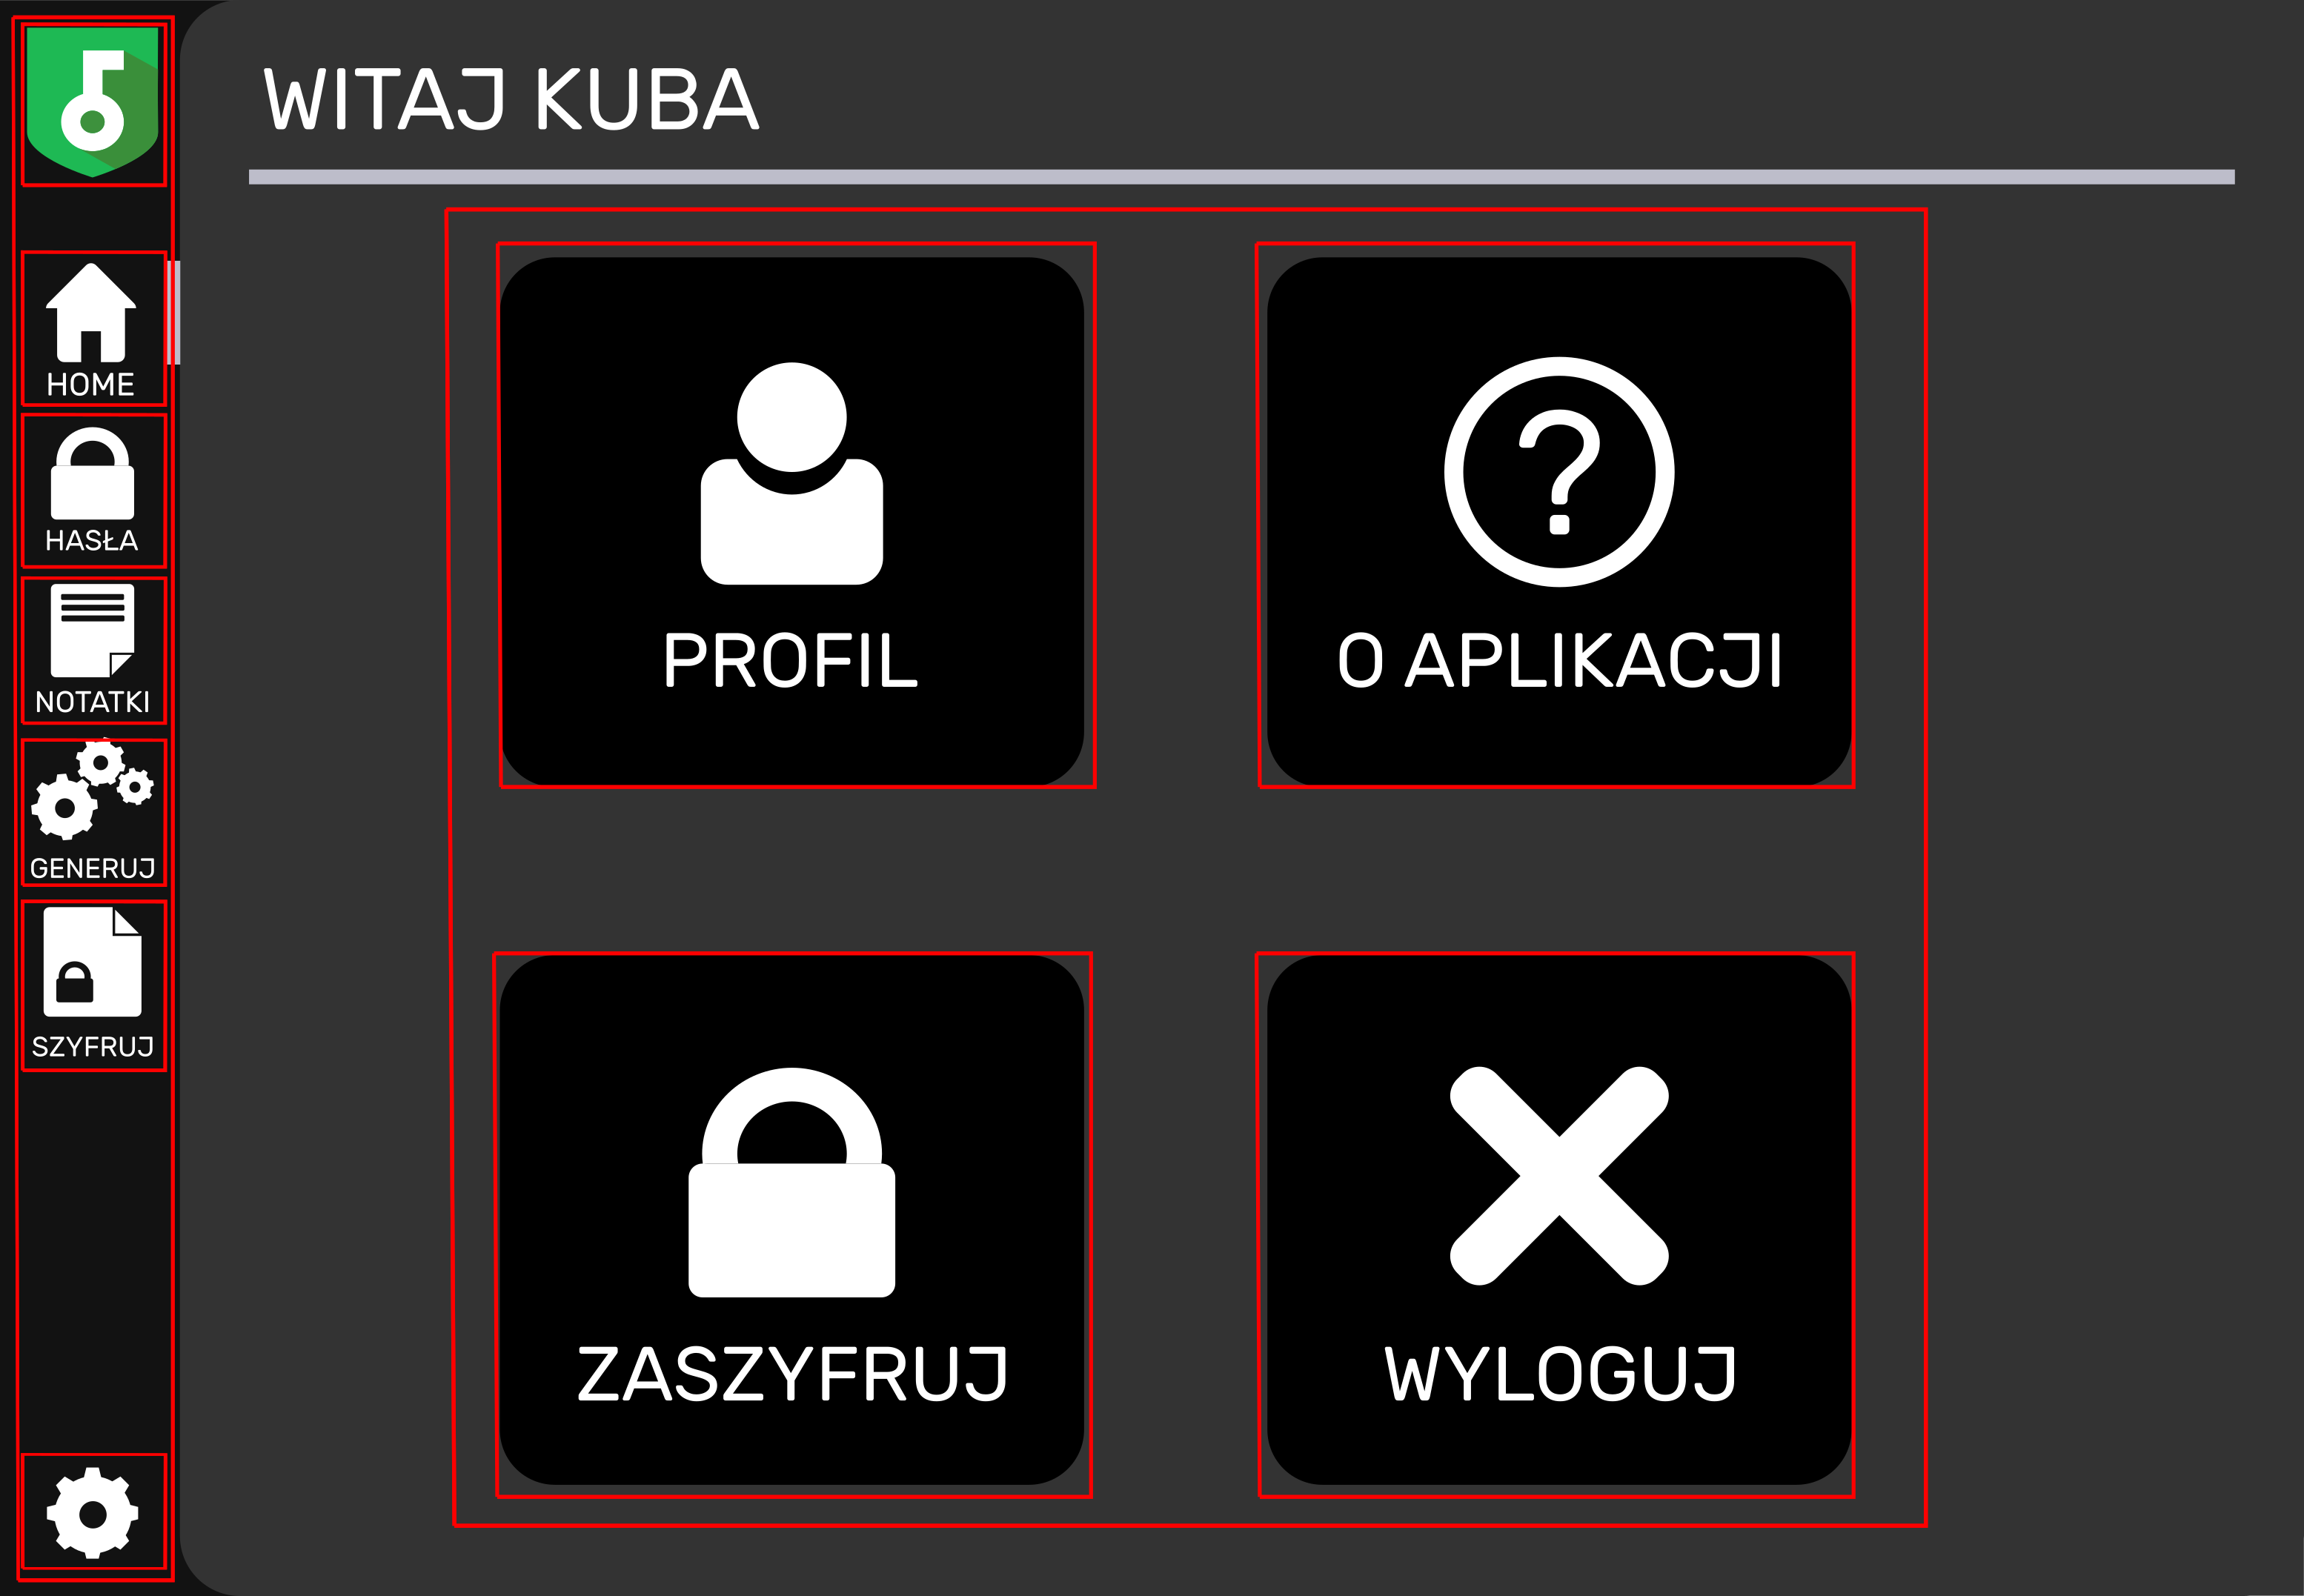
\includegraphics[width=1\textwidth]{img/ekran_przed_zalogowanie.png}
    \caption{Ekran startowy -- przed zalogowaniem}
    \label{fig:startPrzed}
\end{figure}

\begin{figure}[H]
    \centering
    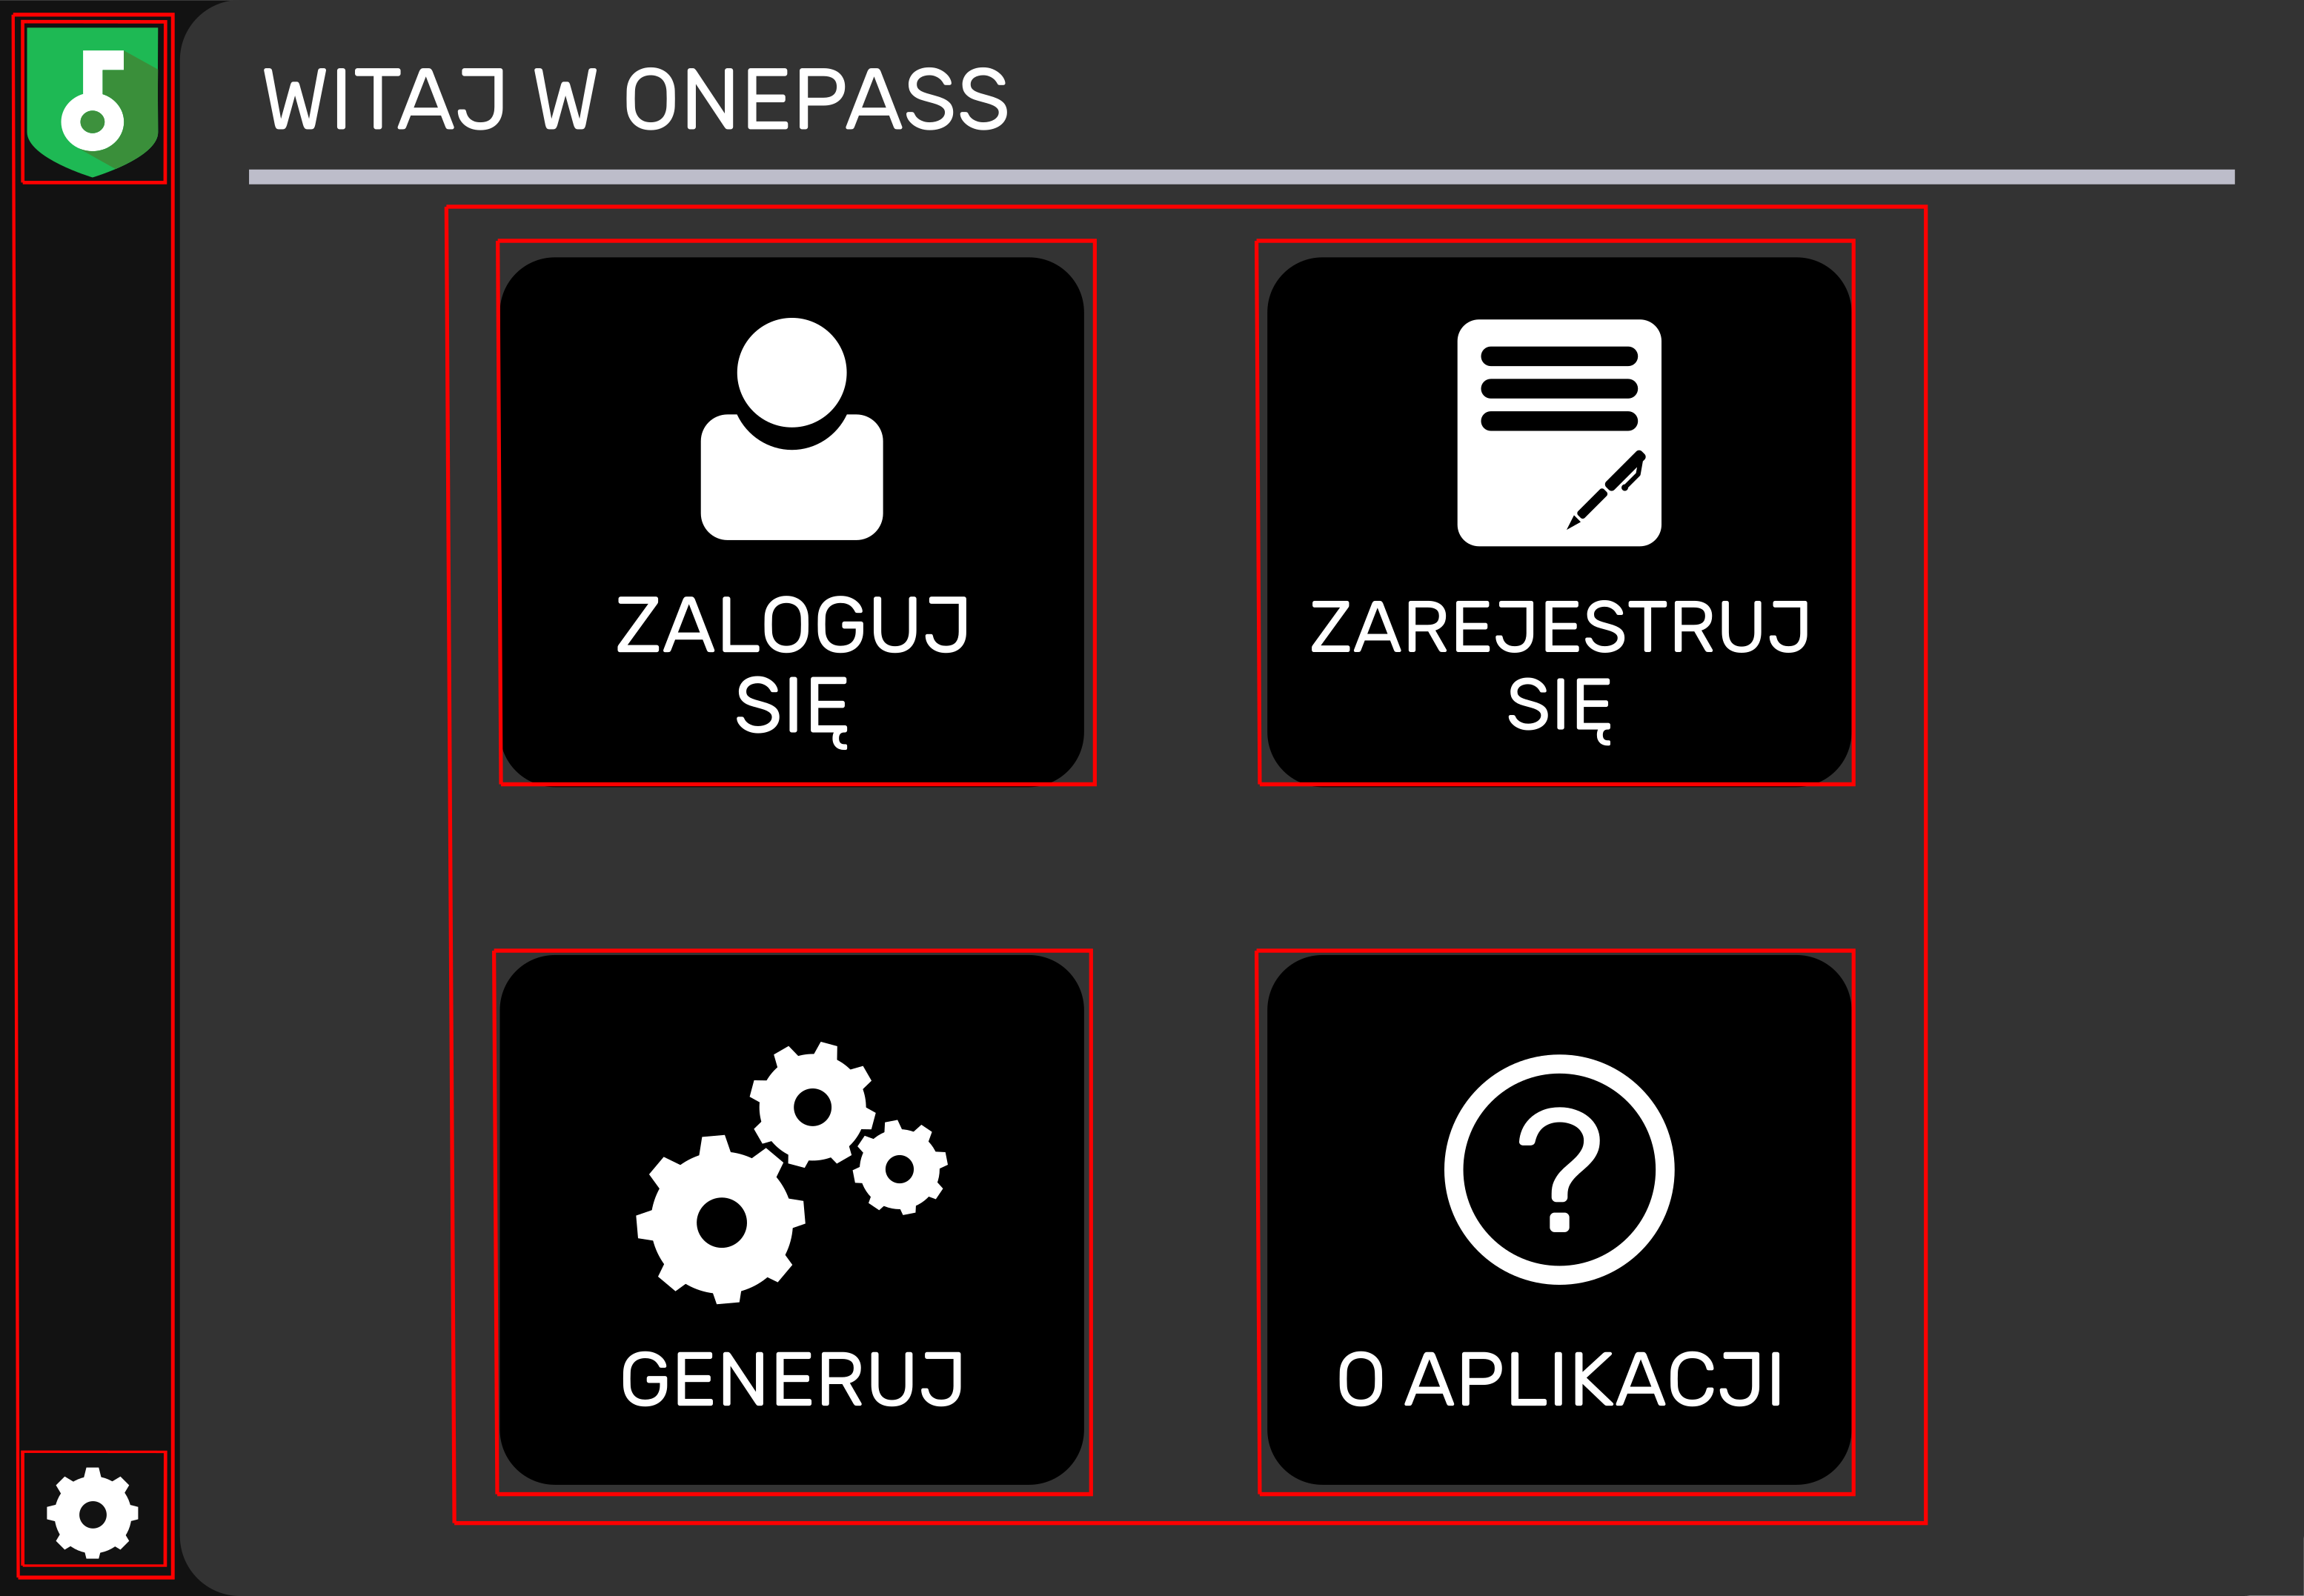
\includegraphics[width=1\textwidth]{img/ekran_po_zalogowanie.png}
    \caption{Ekran startowy -- po zalogowaniu}
    \label{fig:startPo}
\end{figure}

\begin{figure}[H]
    \centering
    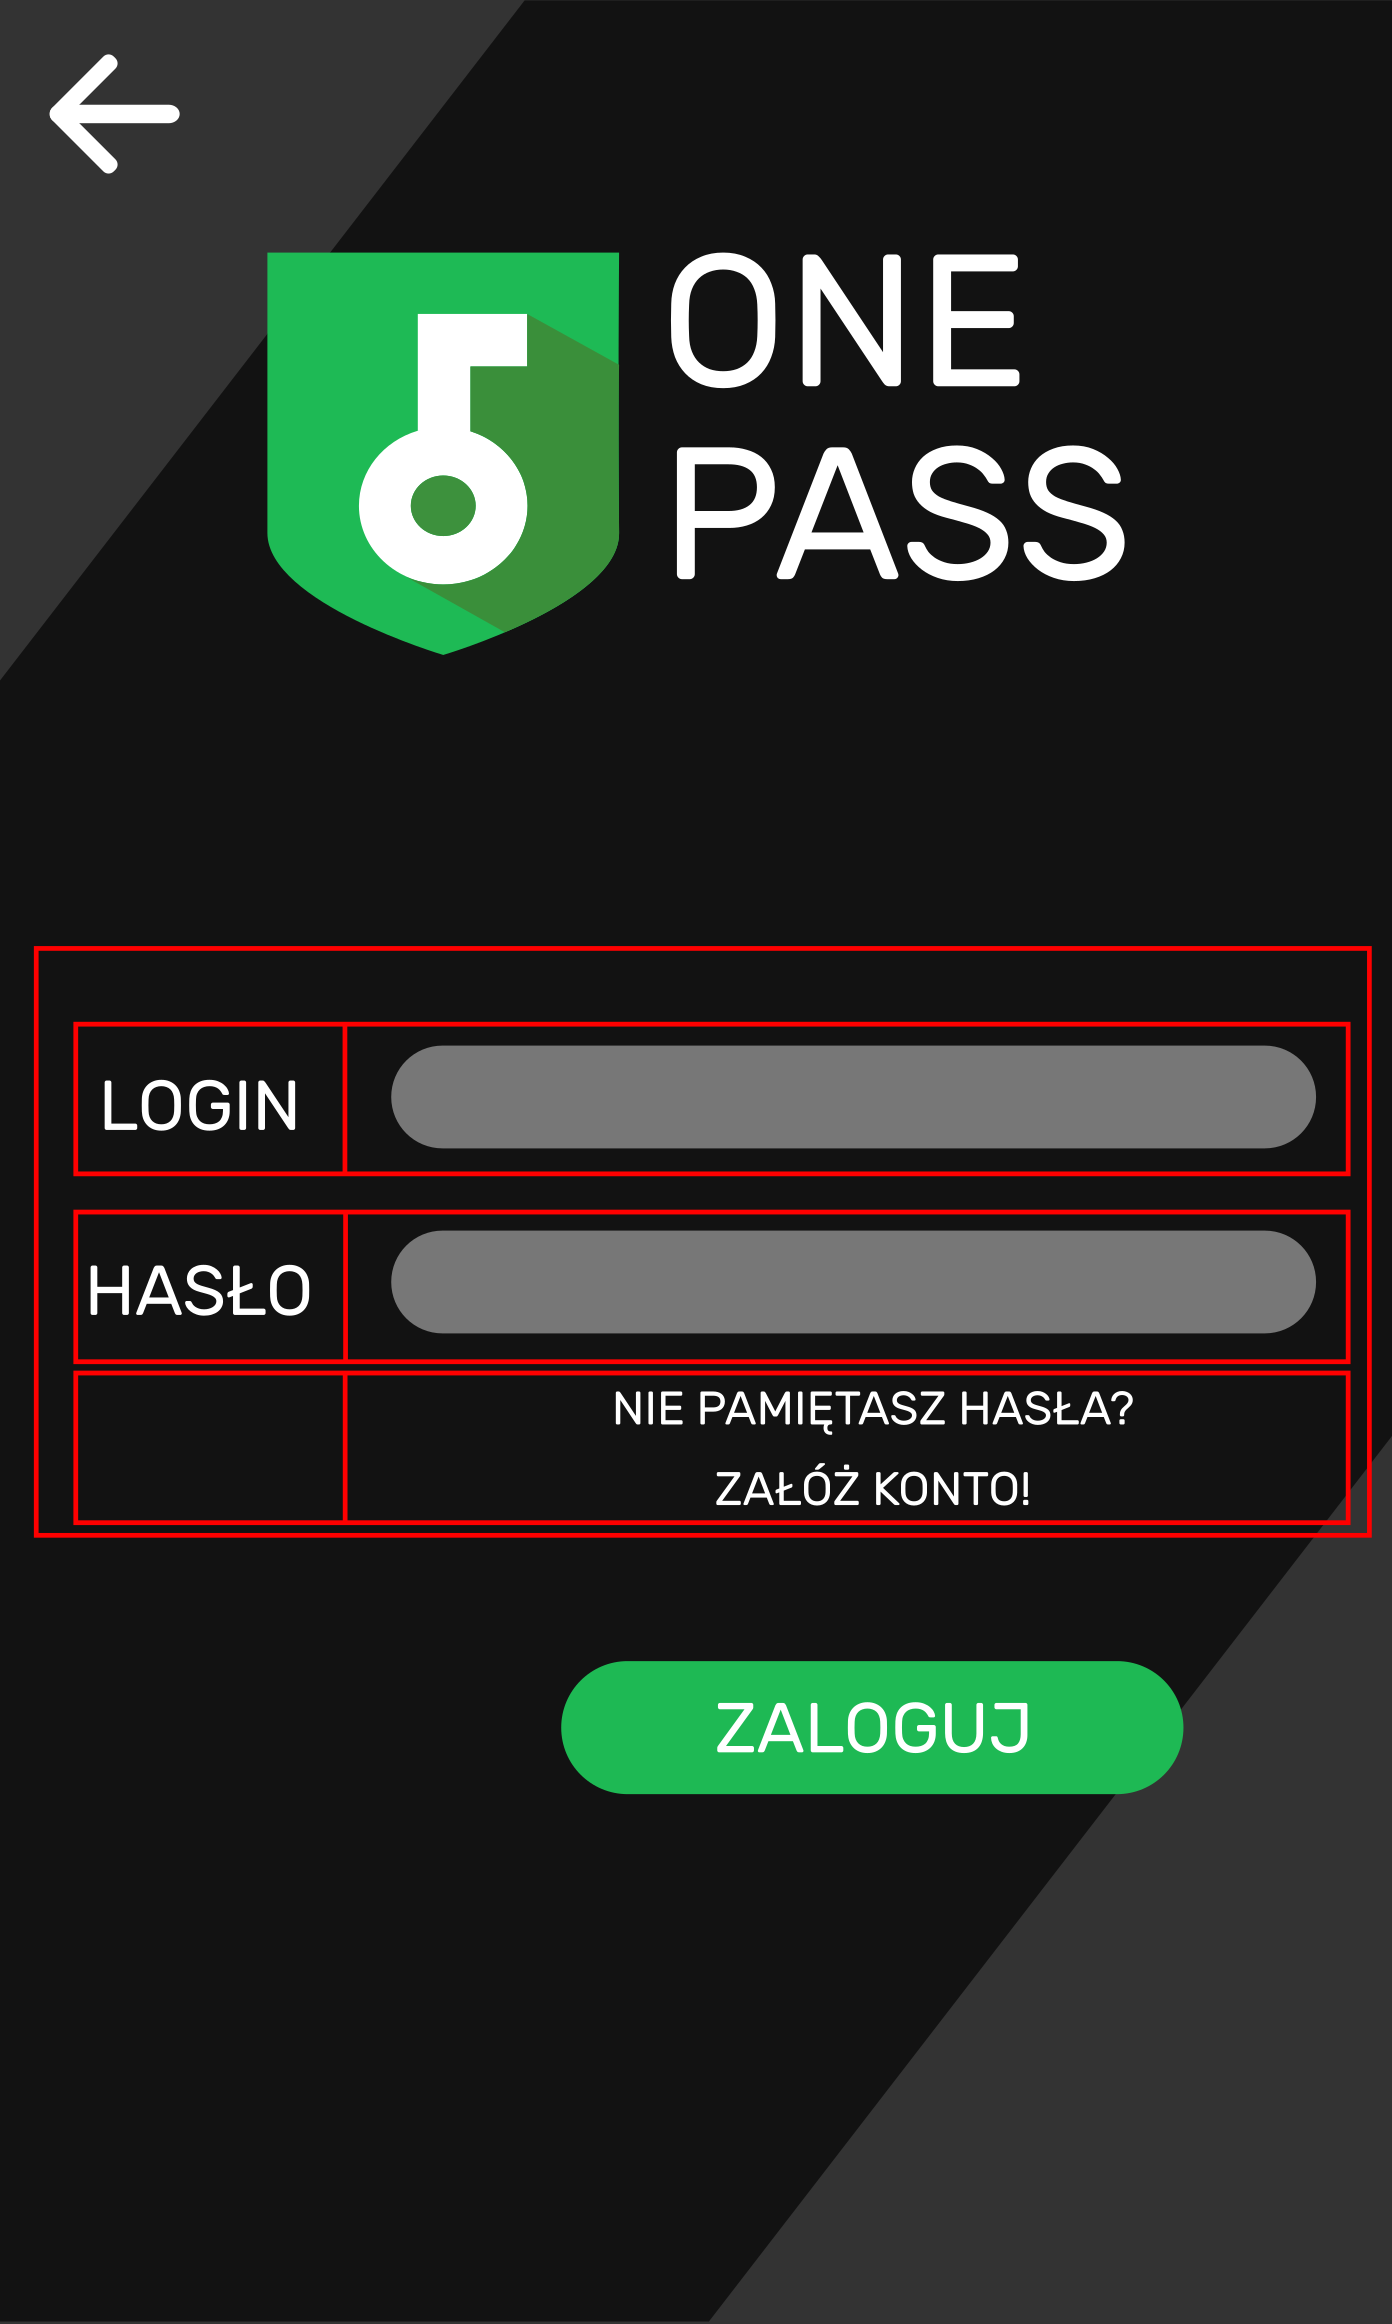
\includegraphics[height=1\textwidth]{img/ekran_logowania.png}
    \caption{Ekran logowania}
    \label{fig:logowanie}
\end{figure}

\begin{figure}[H]
    \centering
    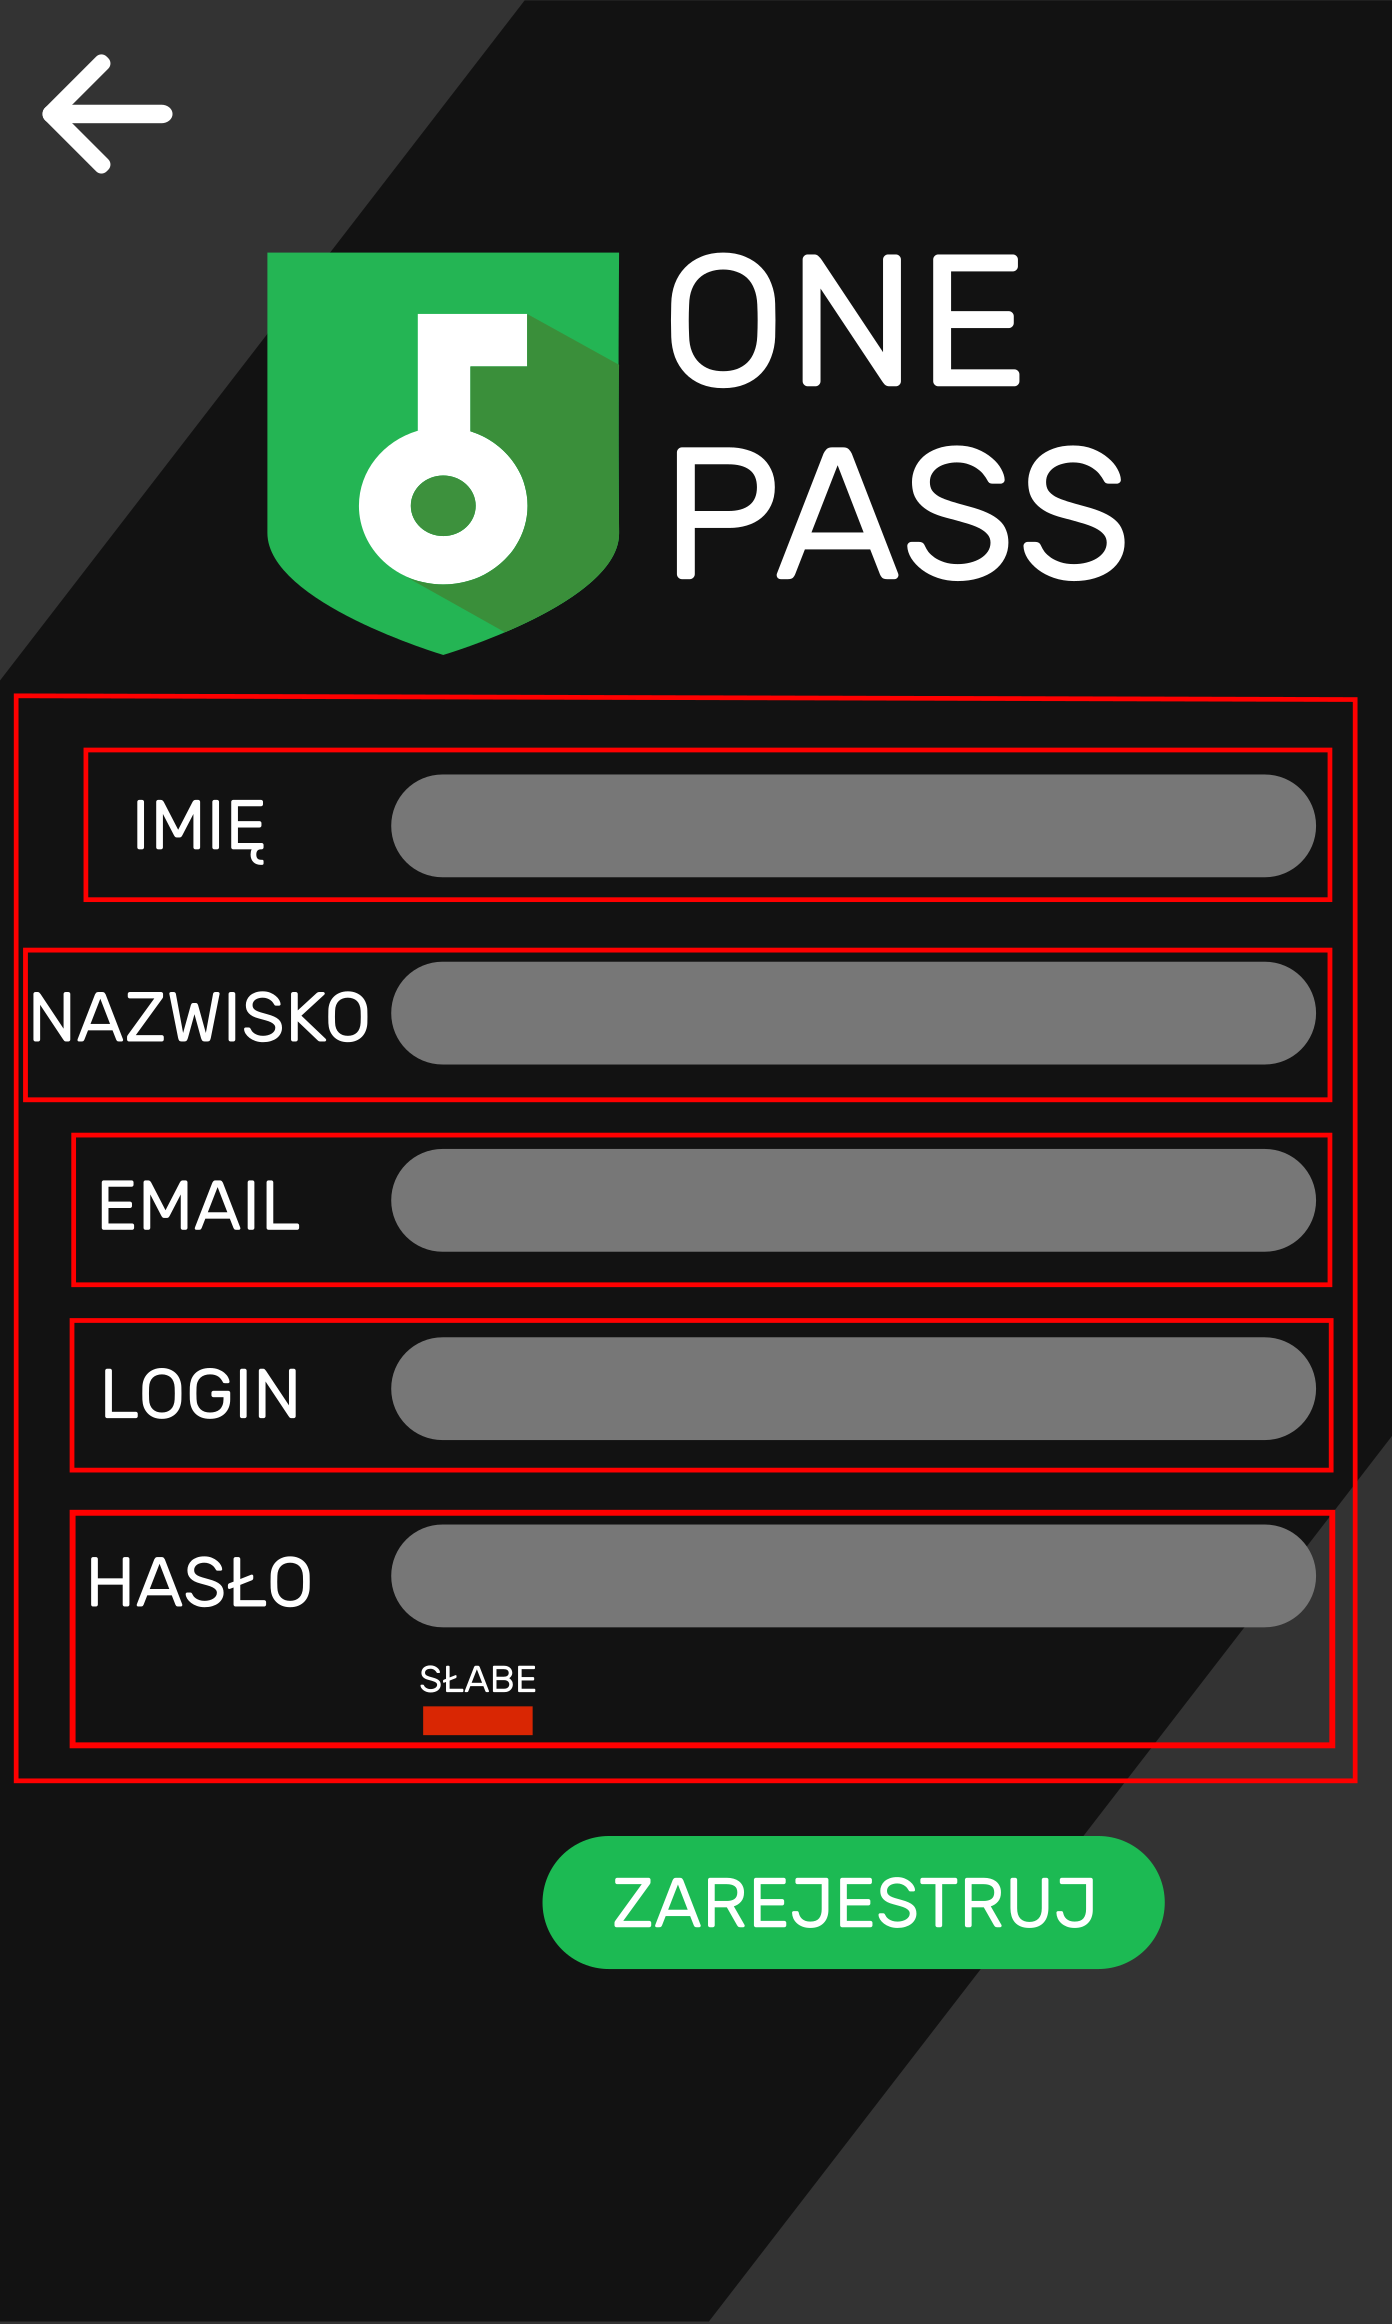
\includegraphics[height=1\textwidth]{img/ekran_rej.png}
    \caption{Ekran rejestracji}
    \label{fig:rejestracja}
\end{figure}

\begin{figure}[H]
    \centering
    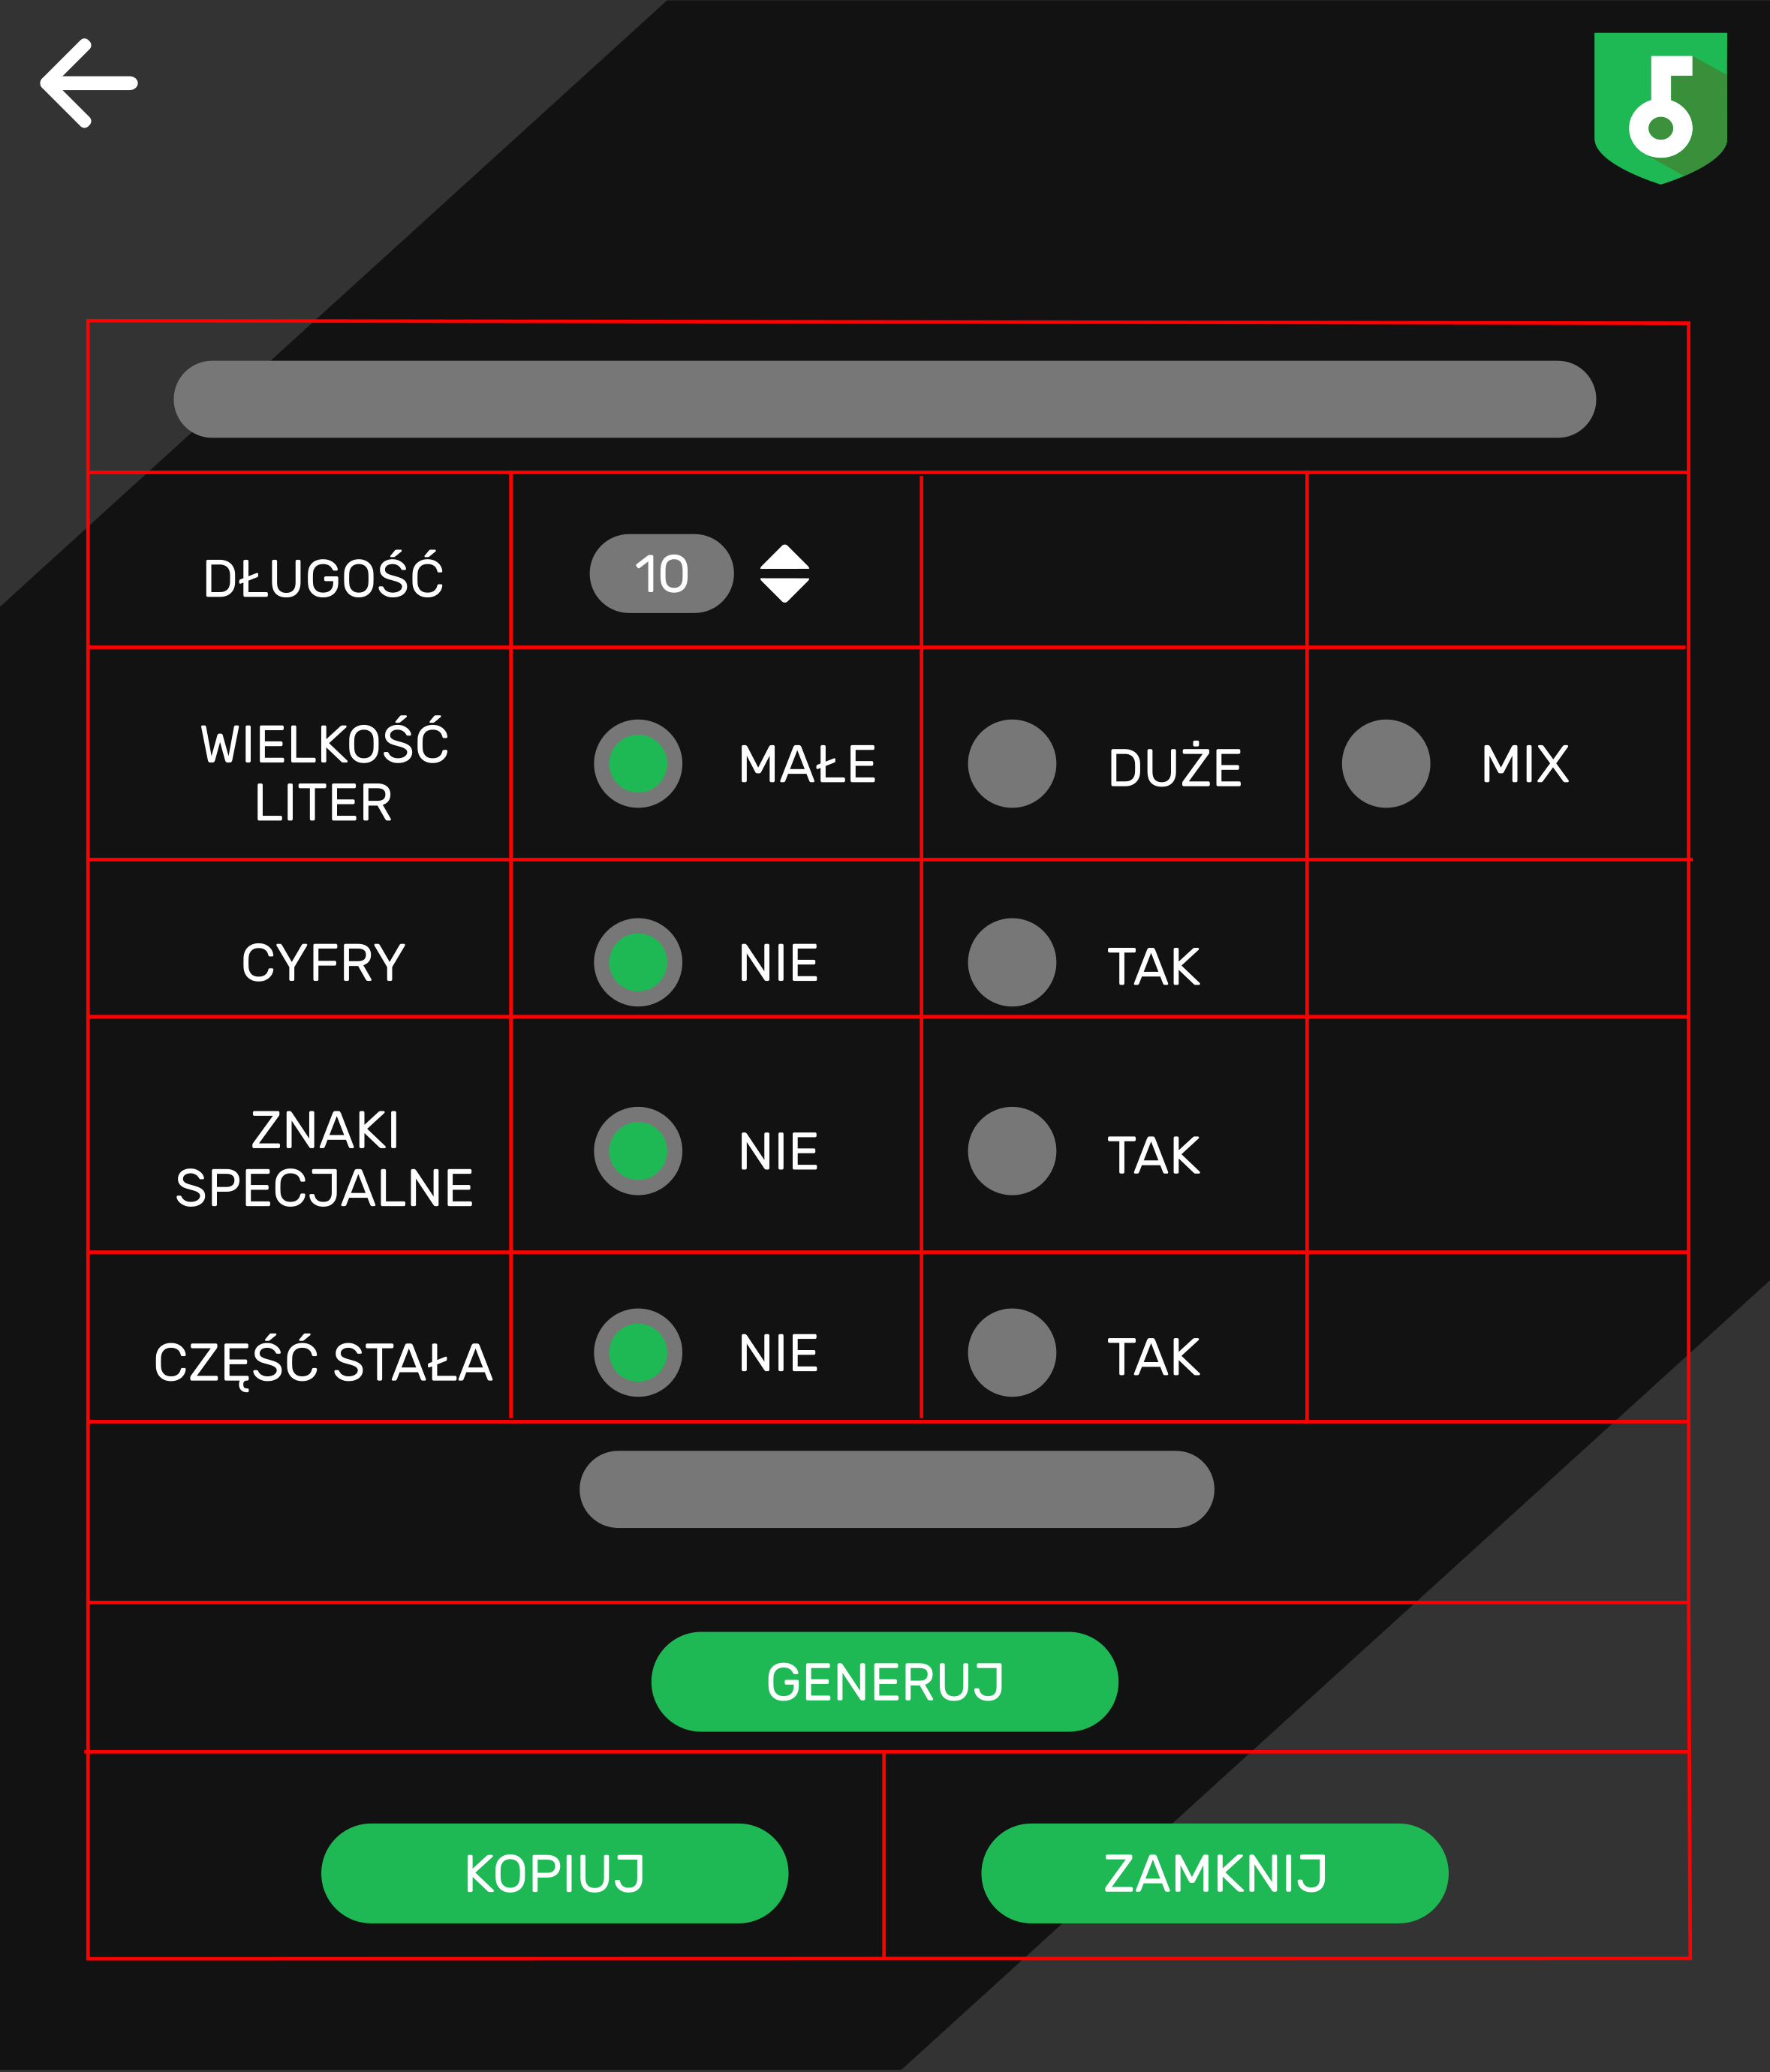
\includegraphics[height=1\textwidth]{img/ekran_generacji.png}
    \caption{Ekran generowania haseł}
    \label{fig:profil}
\end{figure}

\begin{figure}[H]
    \centering
    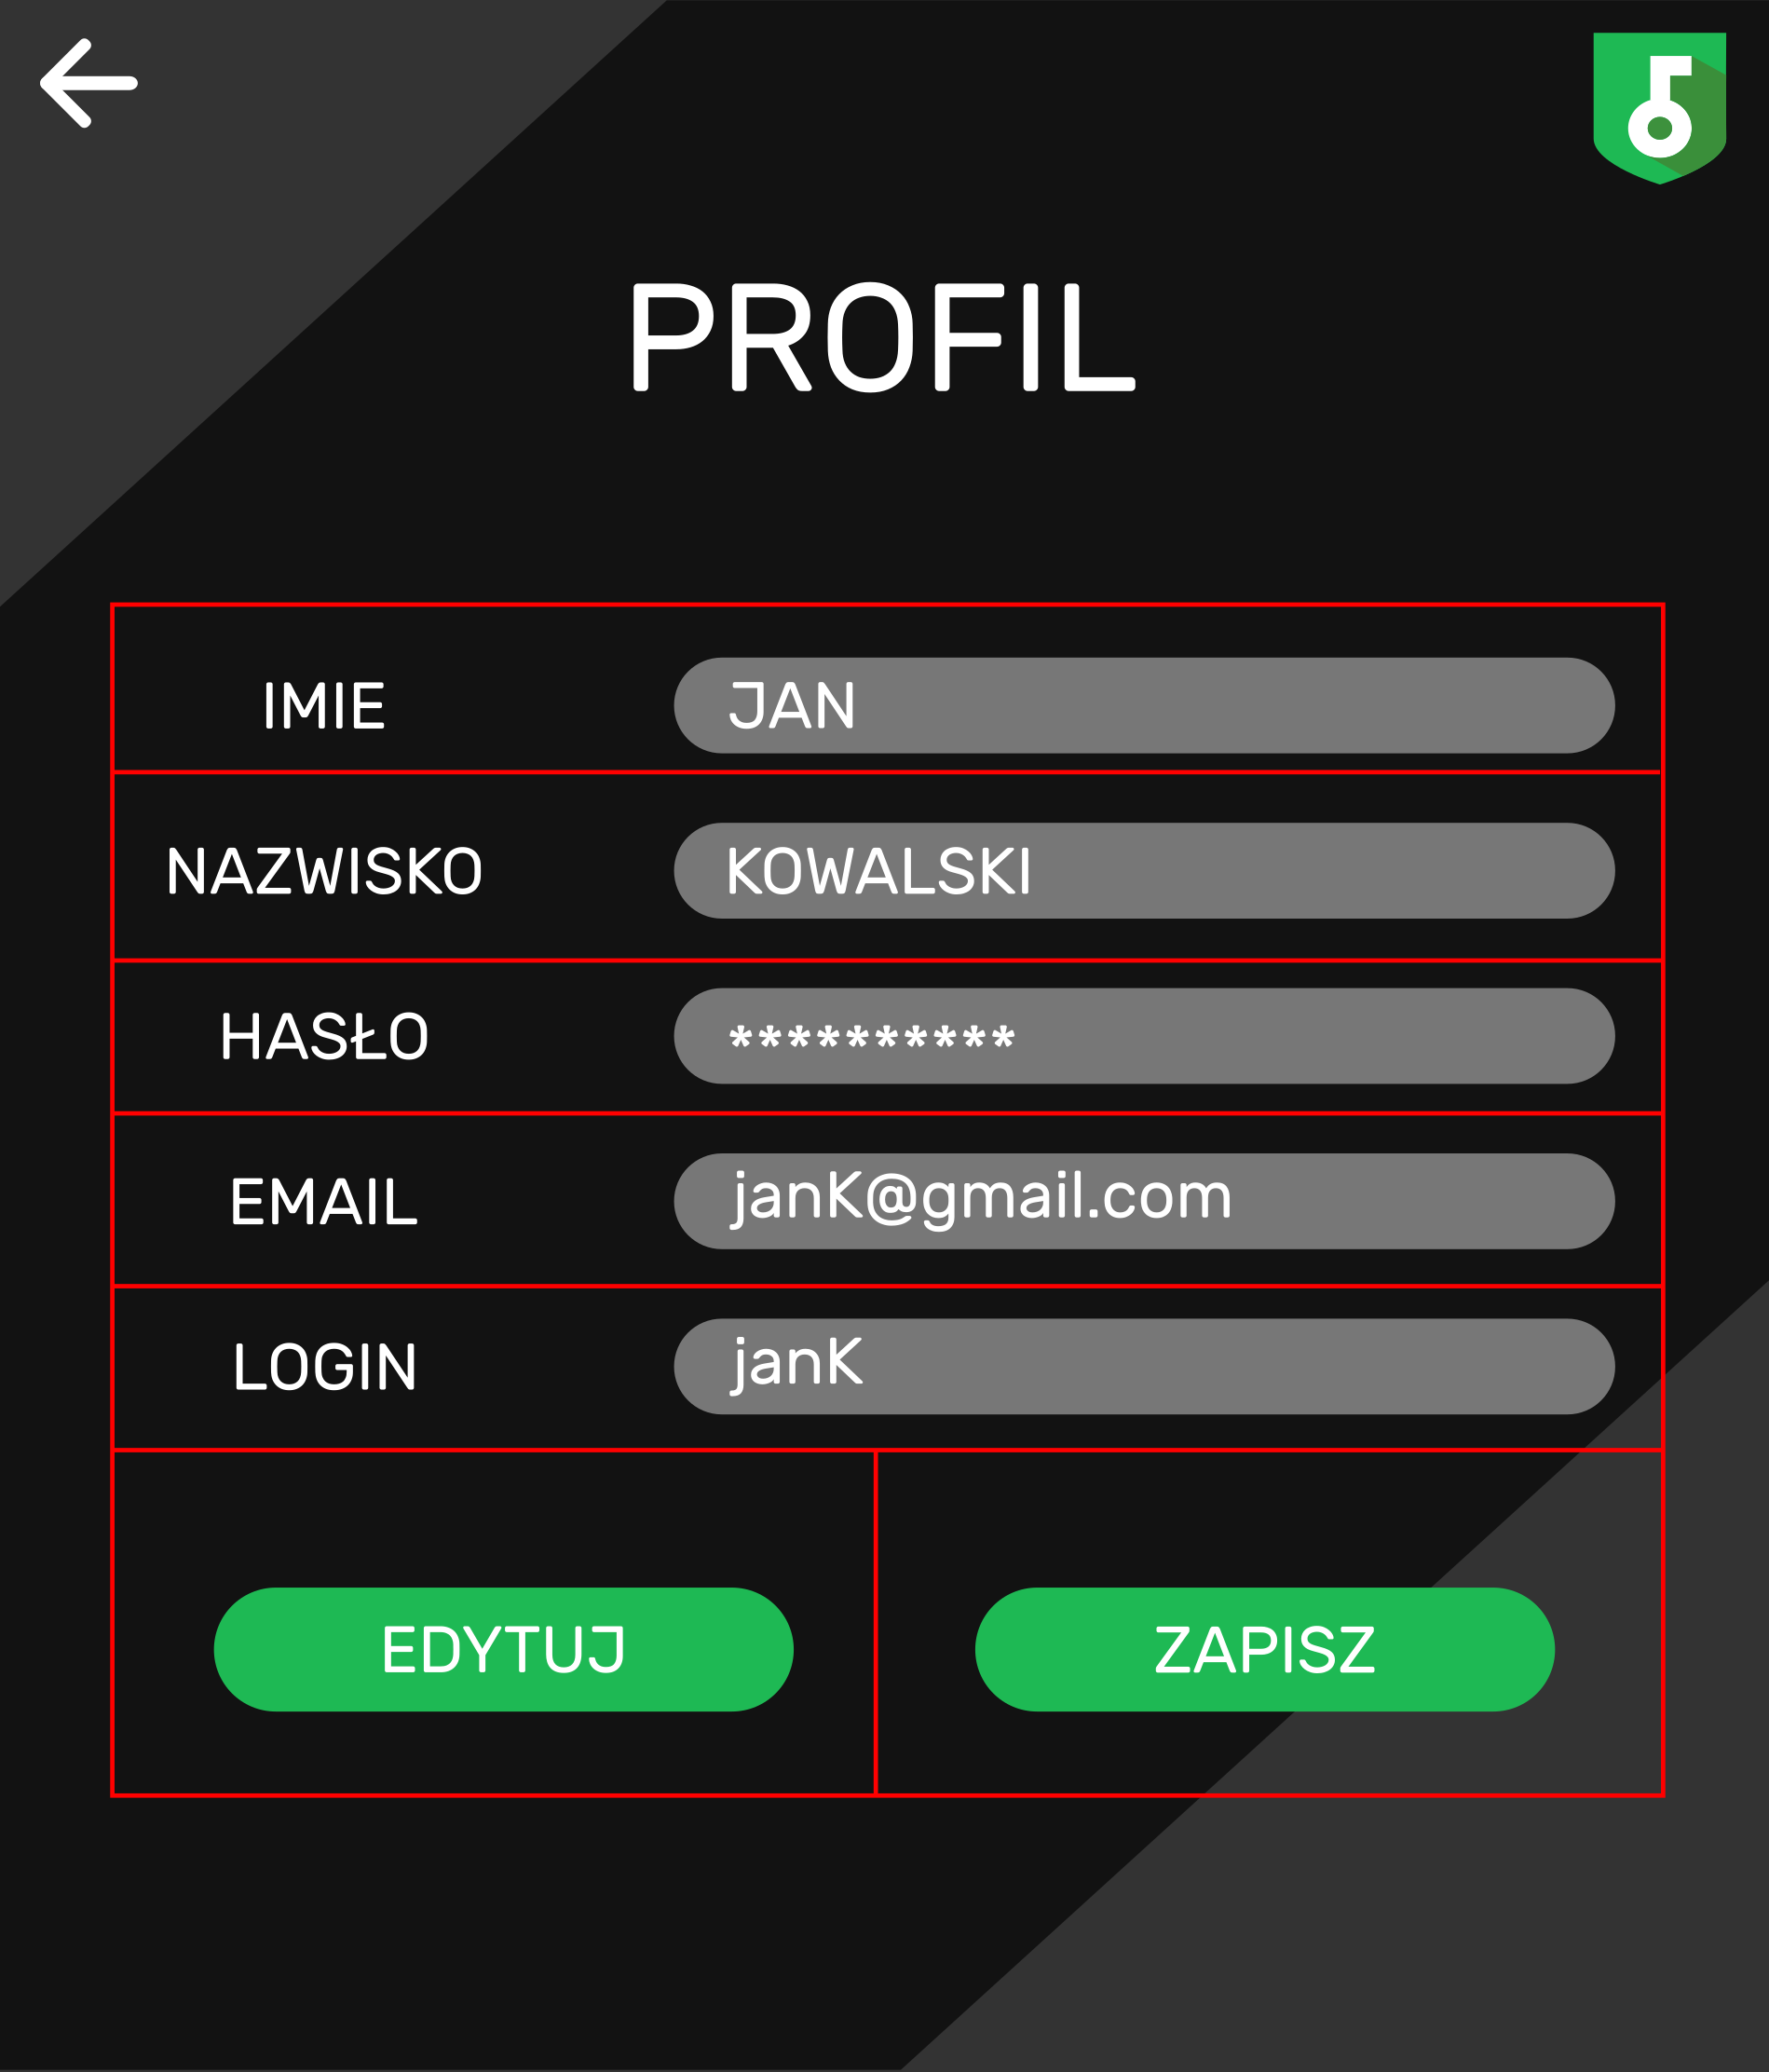
\includegraphics[height=1\textwidth]{img/ekran_profilu.png}
    \caption{Ekran informacji o profilu}
    \label{fig:profil}
\end{figure}

\begin{figure}[H]
    \centering
    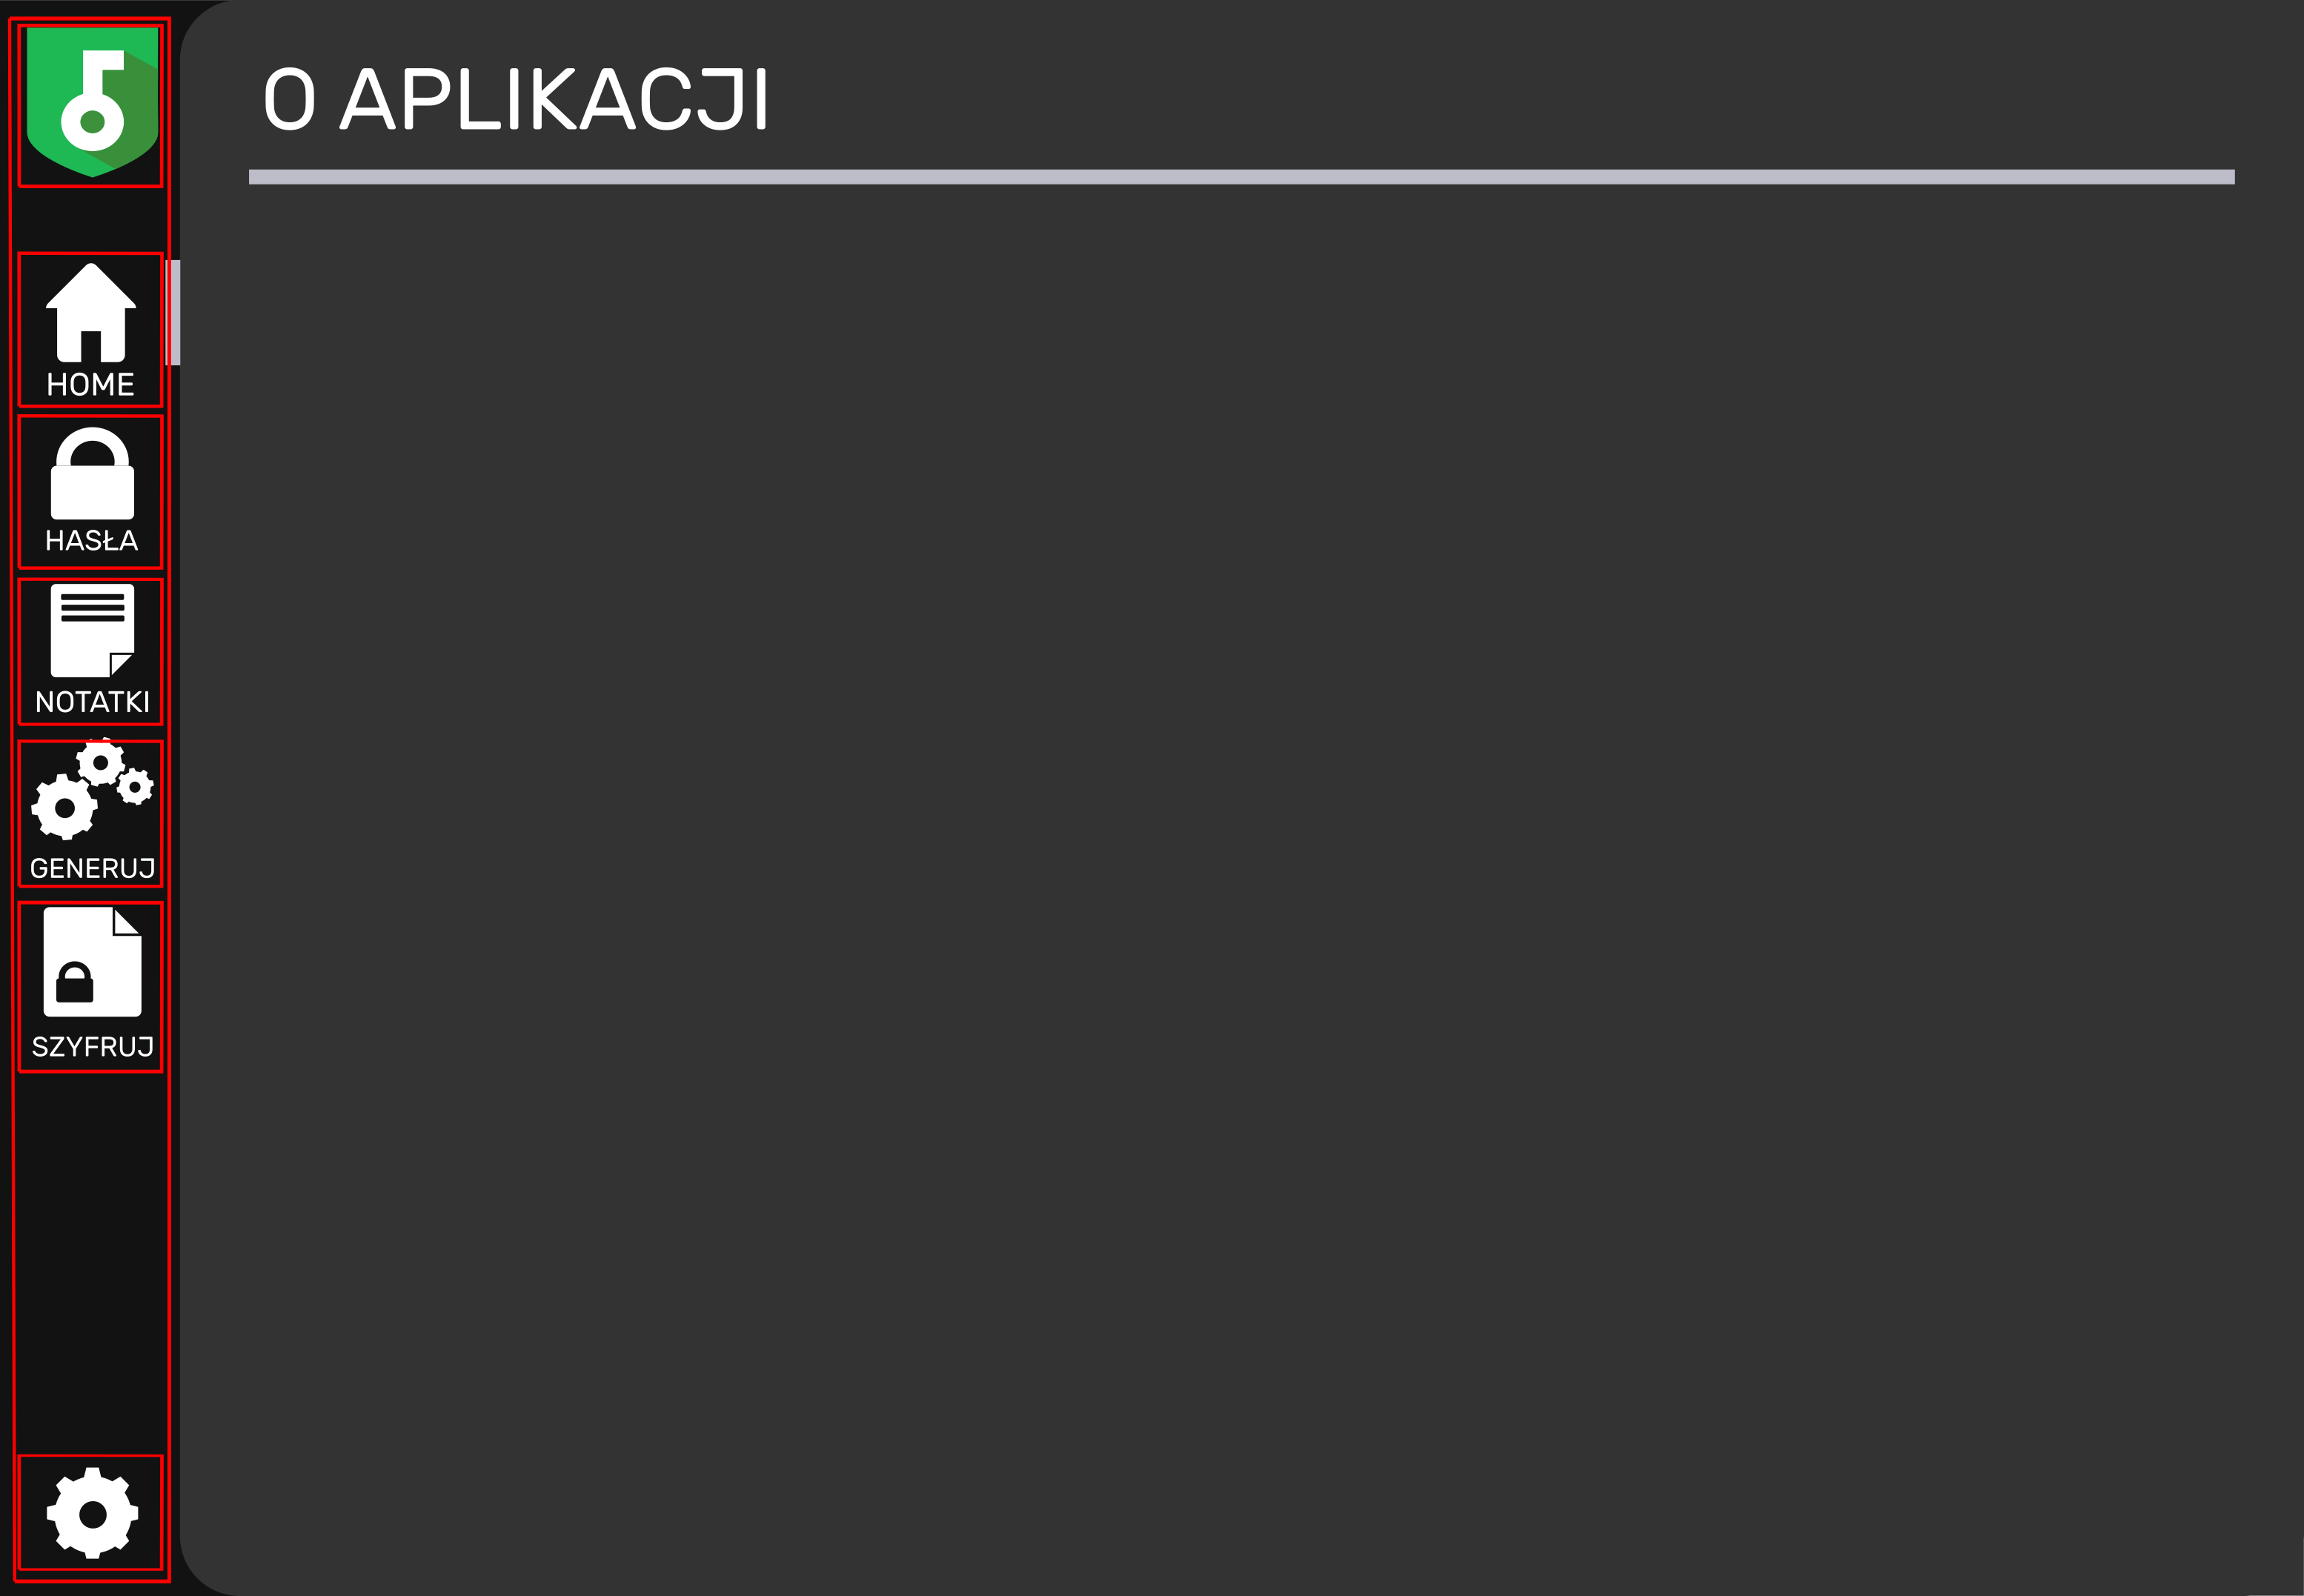
\includegraphics[height=1\textwidth]{img/ekarn_oapp.png}
    \caption{Ekran o aplikacji}
    \label{fig:oApp}
\end{figure}

\begin{figure}[H]
    \centering
    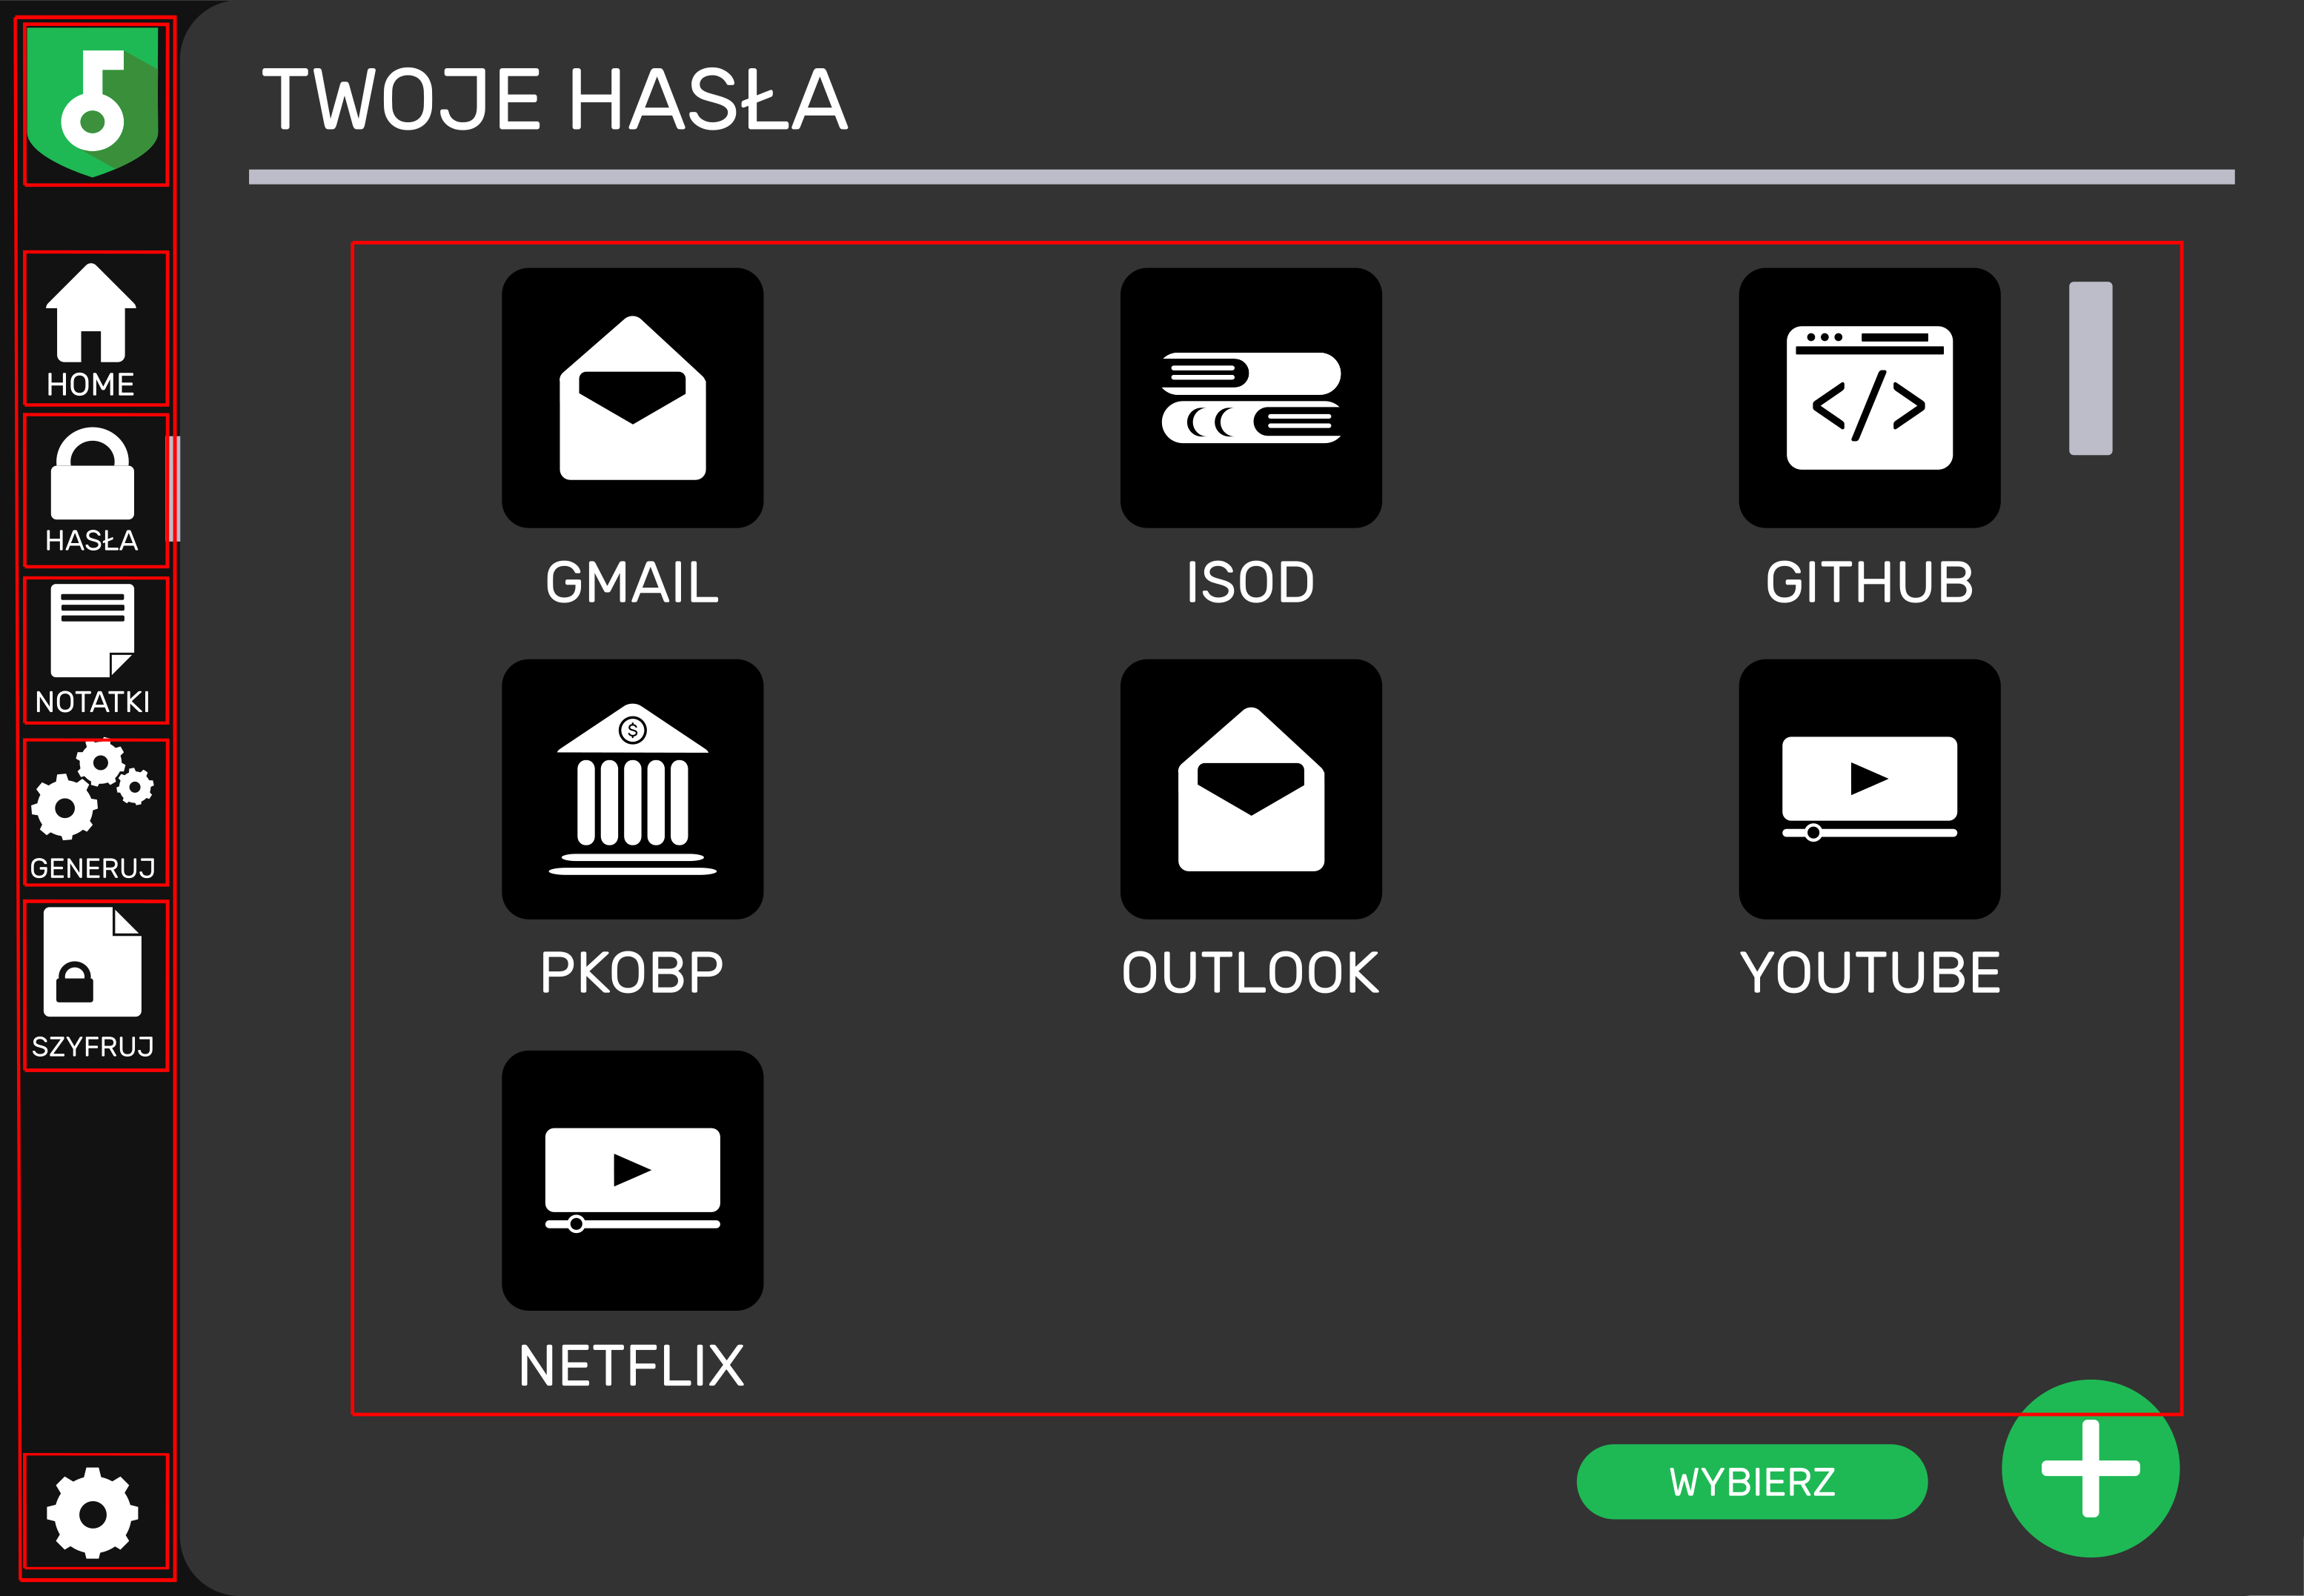
\includegraphics[width=1\textwidth]{img/ekran_hasel.png}
    \caption{Ekran haseł}
    \label{fig:hasla}
\end{figure}

\begin{figure}[H]
    \centering
    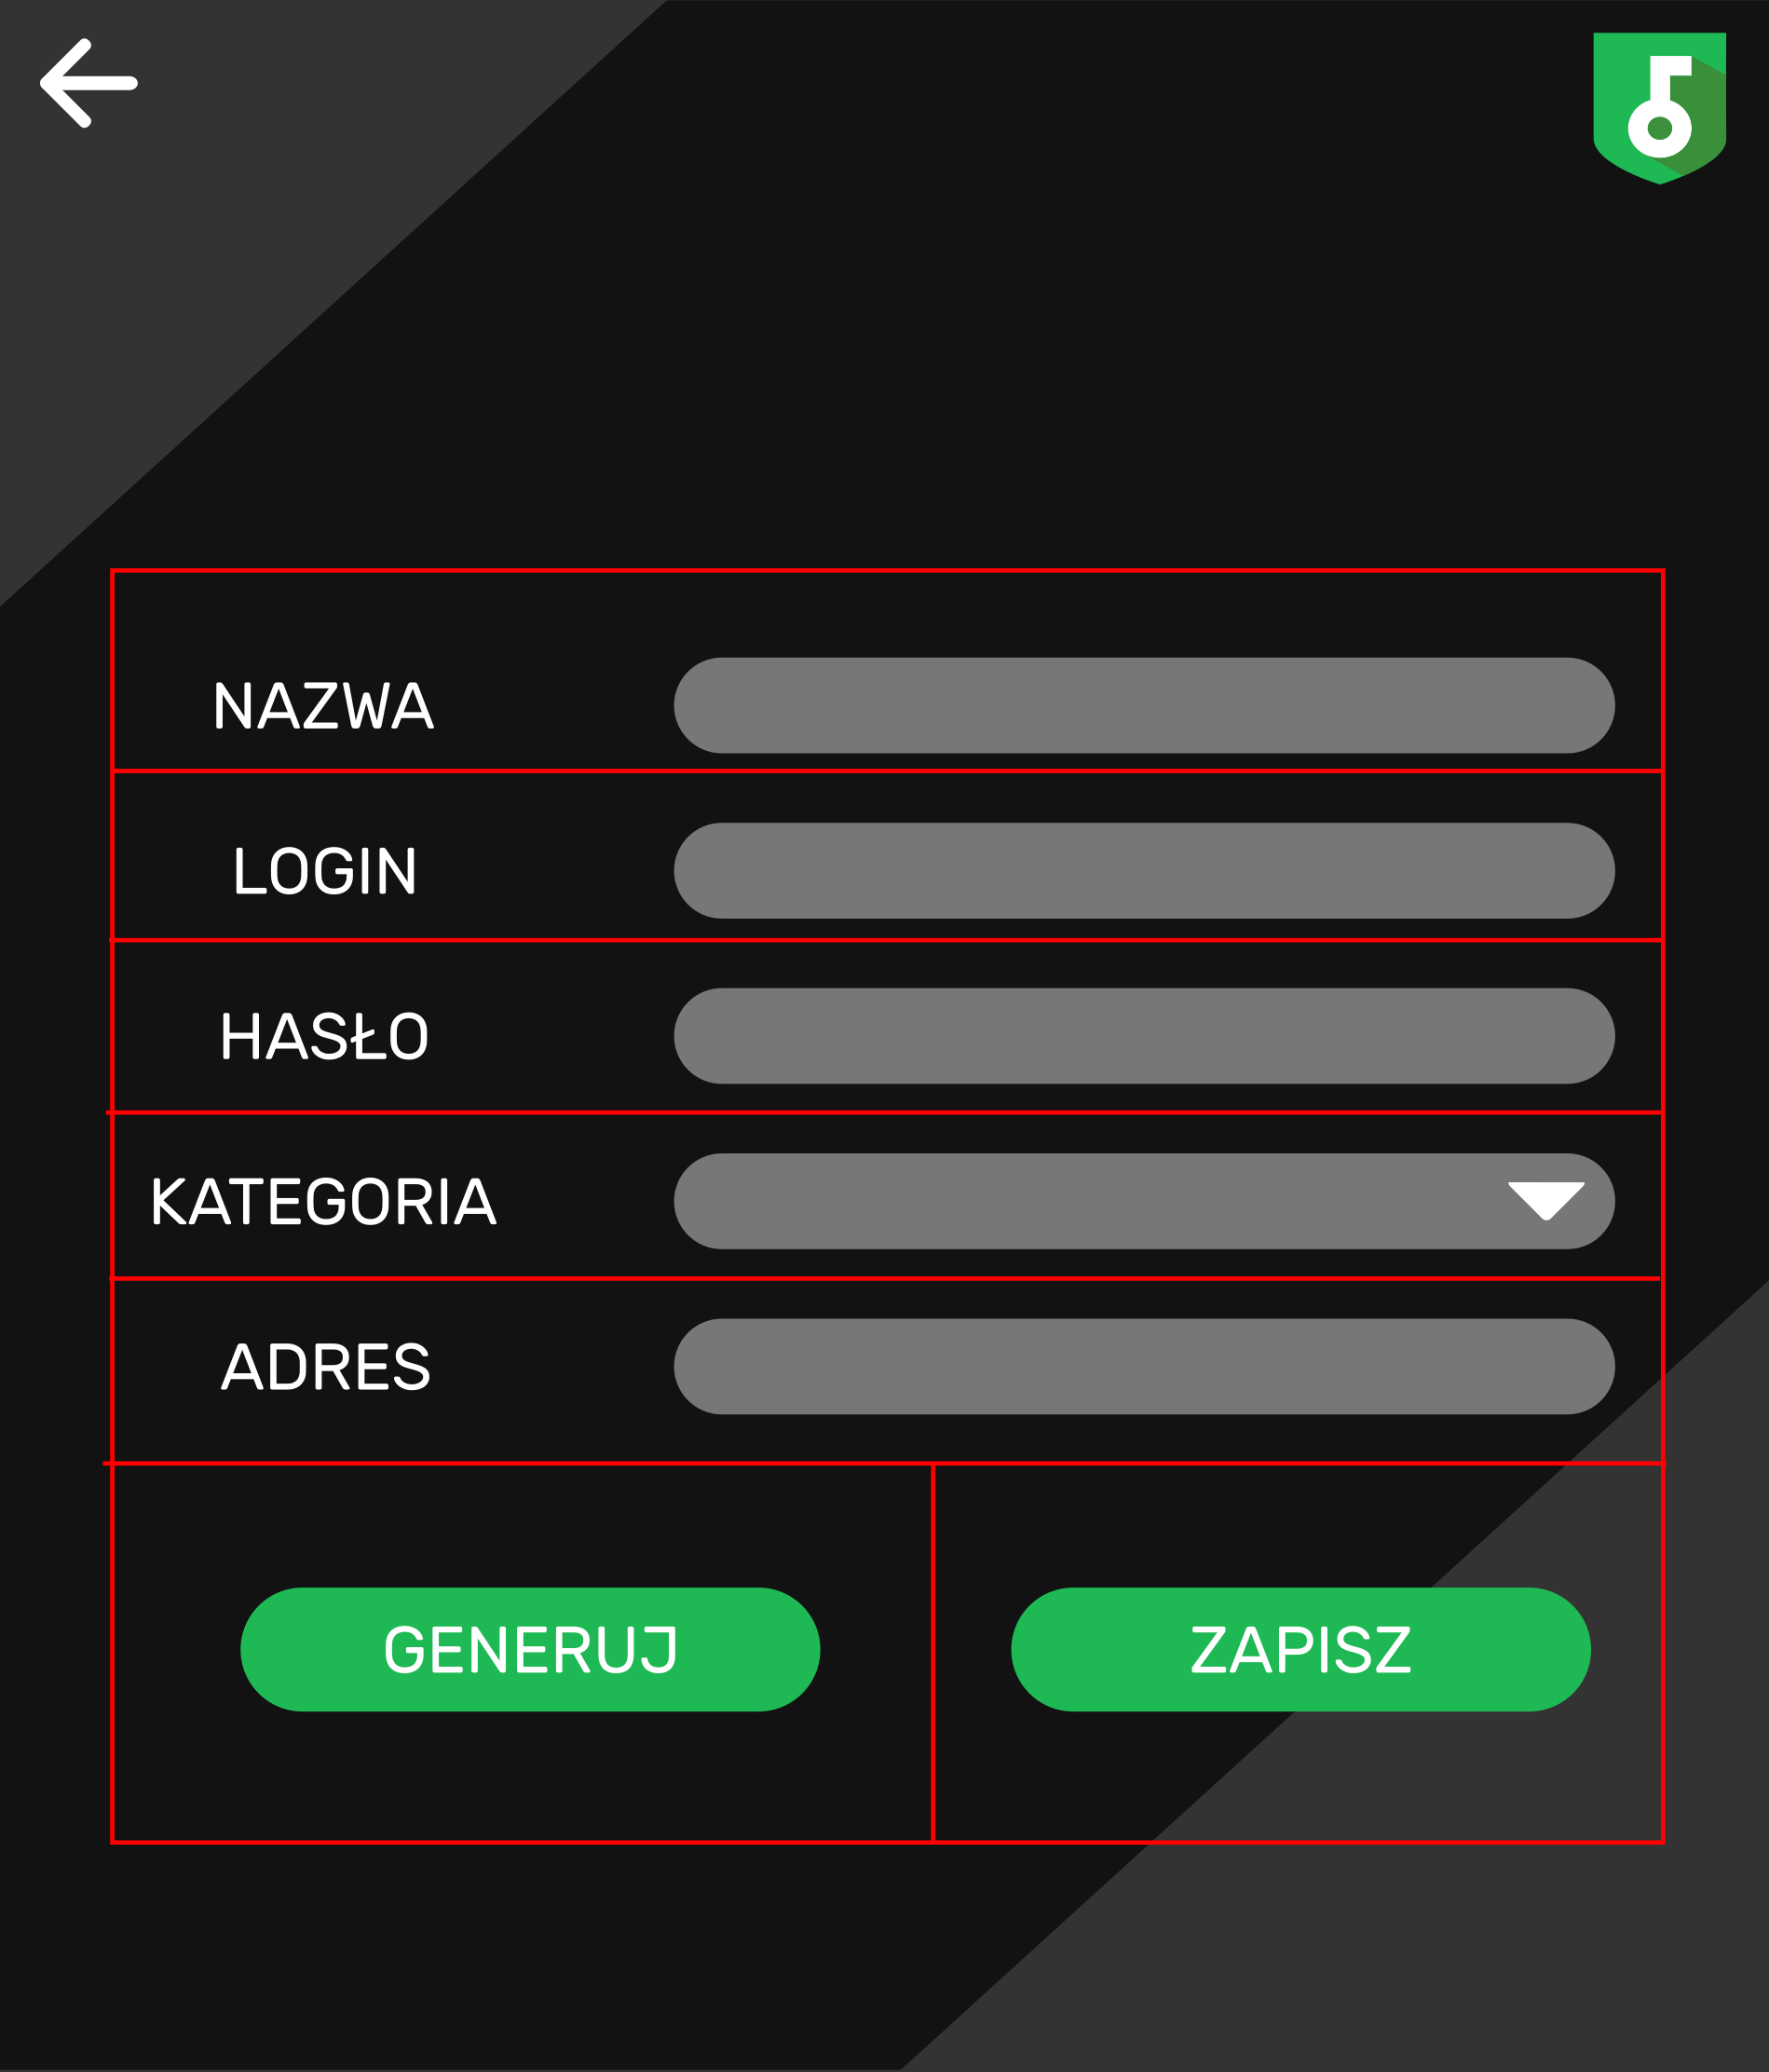
\includegraphics[height=1\textwidth]{img/ekran_dodania.png}
    \caption{Ekran dodawania obiektu}
    \label{fig:haslaDodanie}
\end{figure}

\begin{figure}[H]
    \centering
    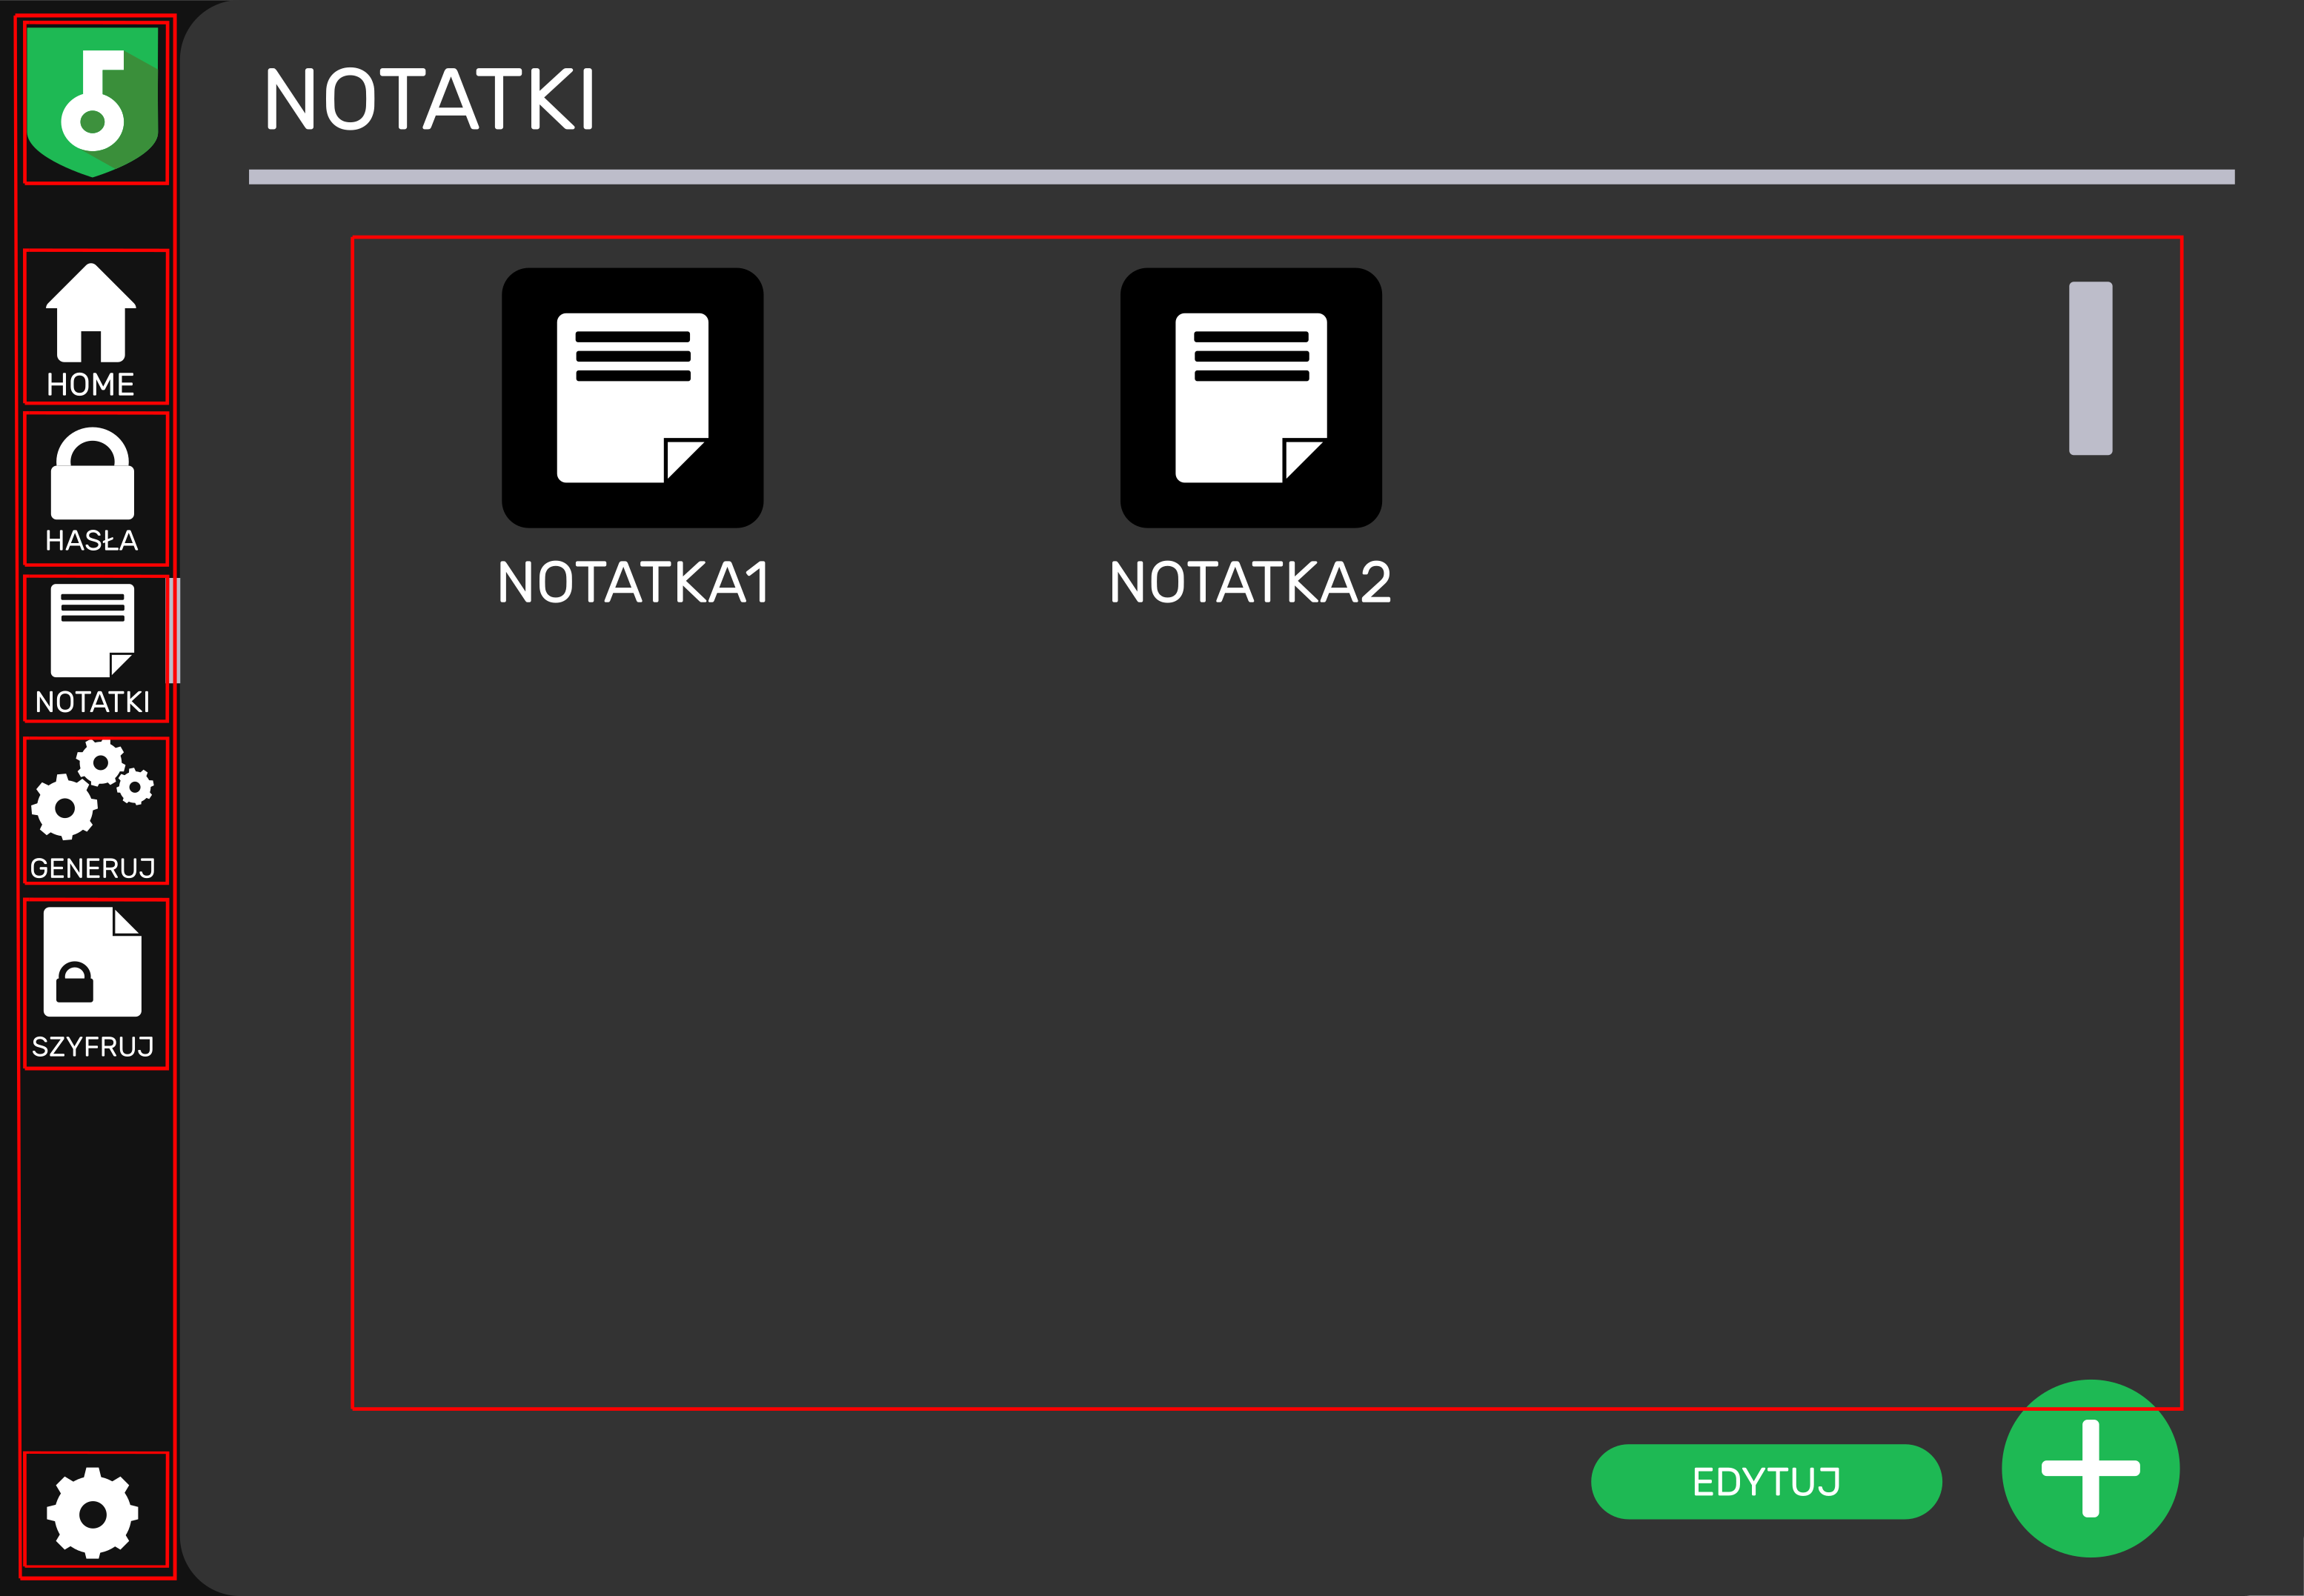
\includegraphics[width=1\textwidth]{img/ekran_notatek.png}
    \caption{Ekran listy notatek}
    \label{fig:notatki}
\end{figure}

\begin{figure}[H]
    \centering
    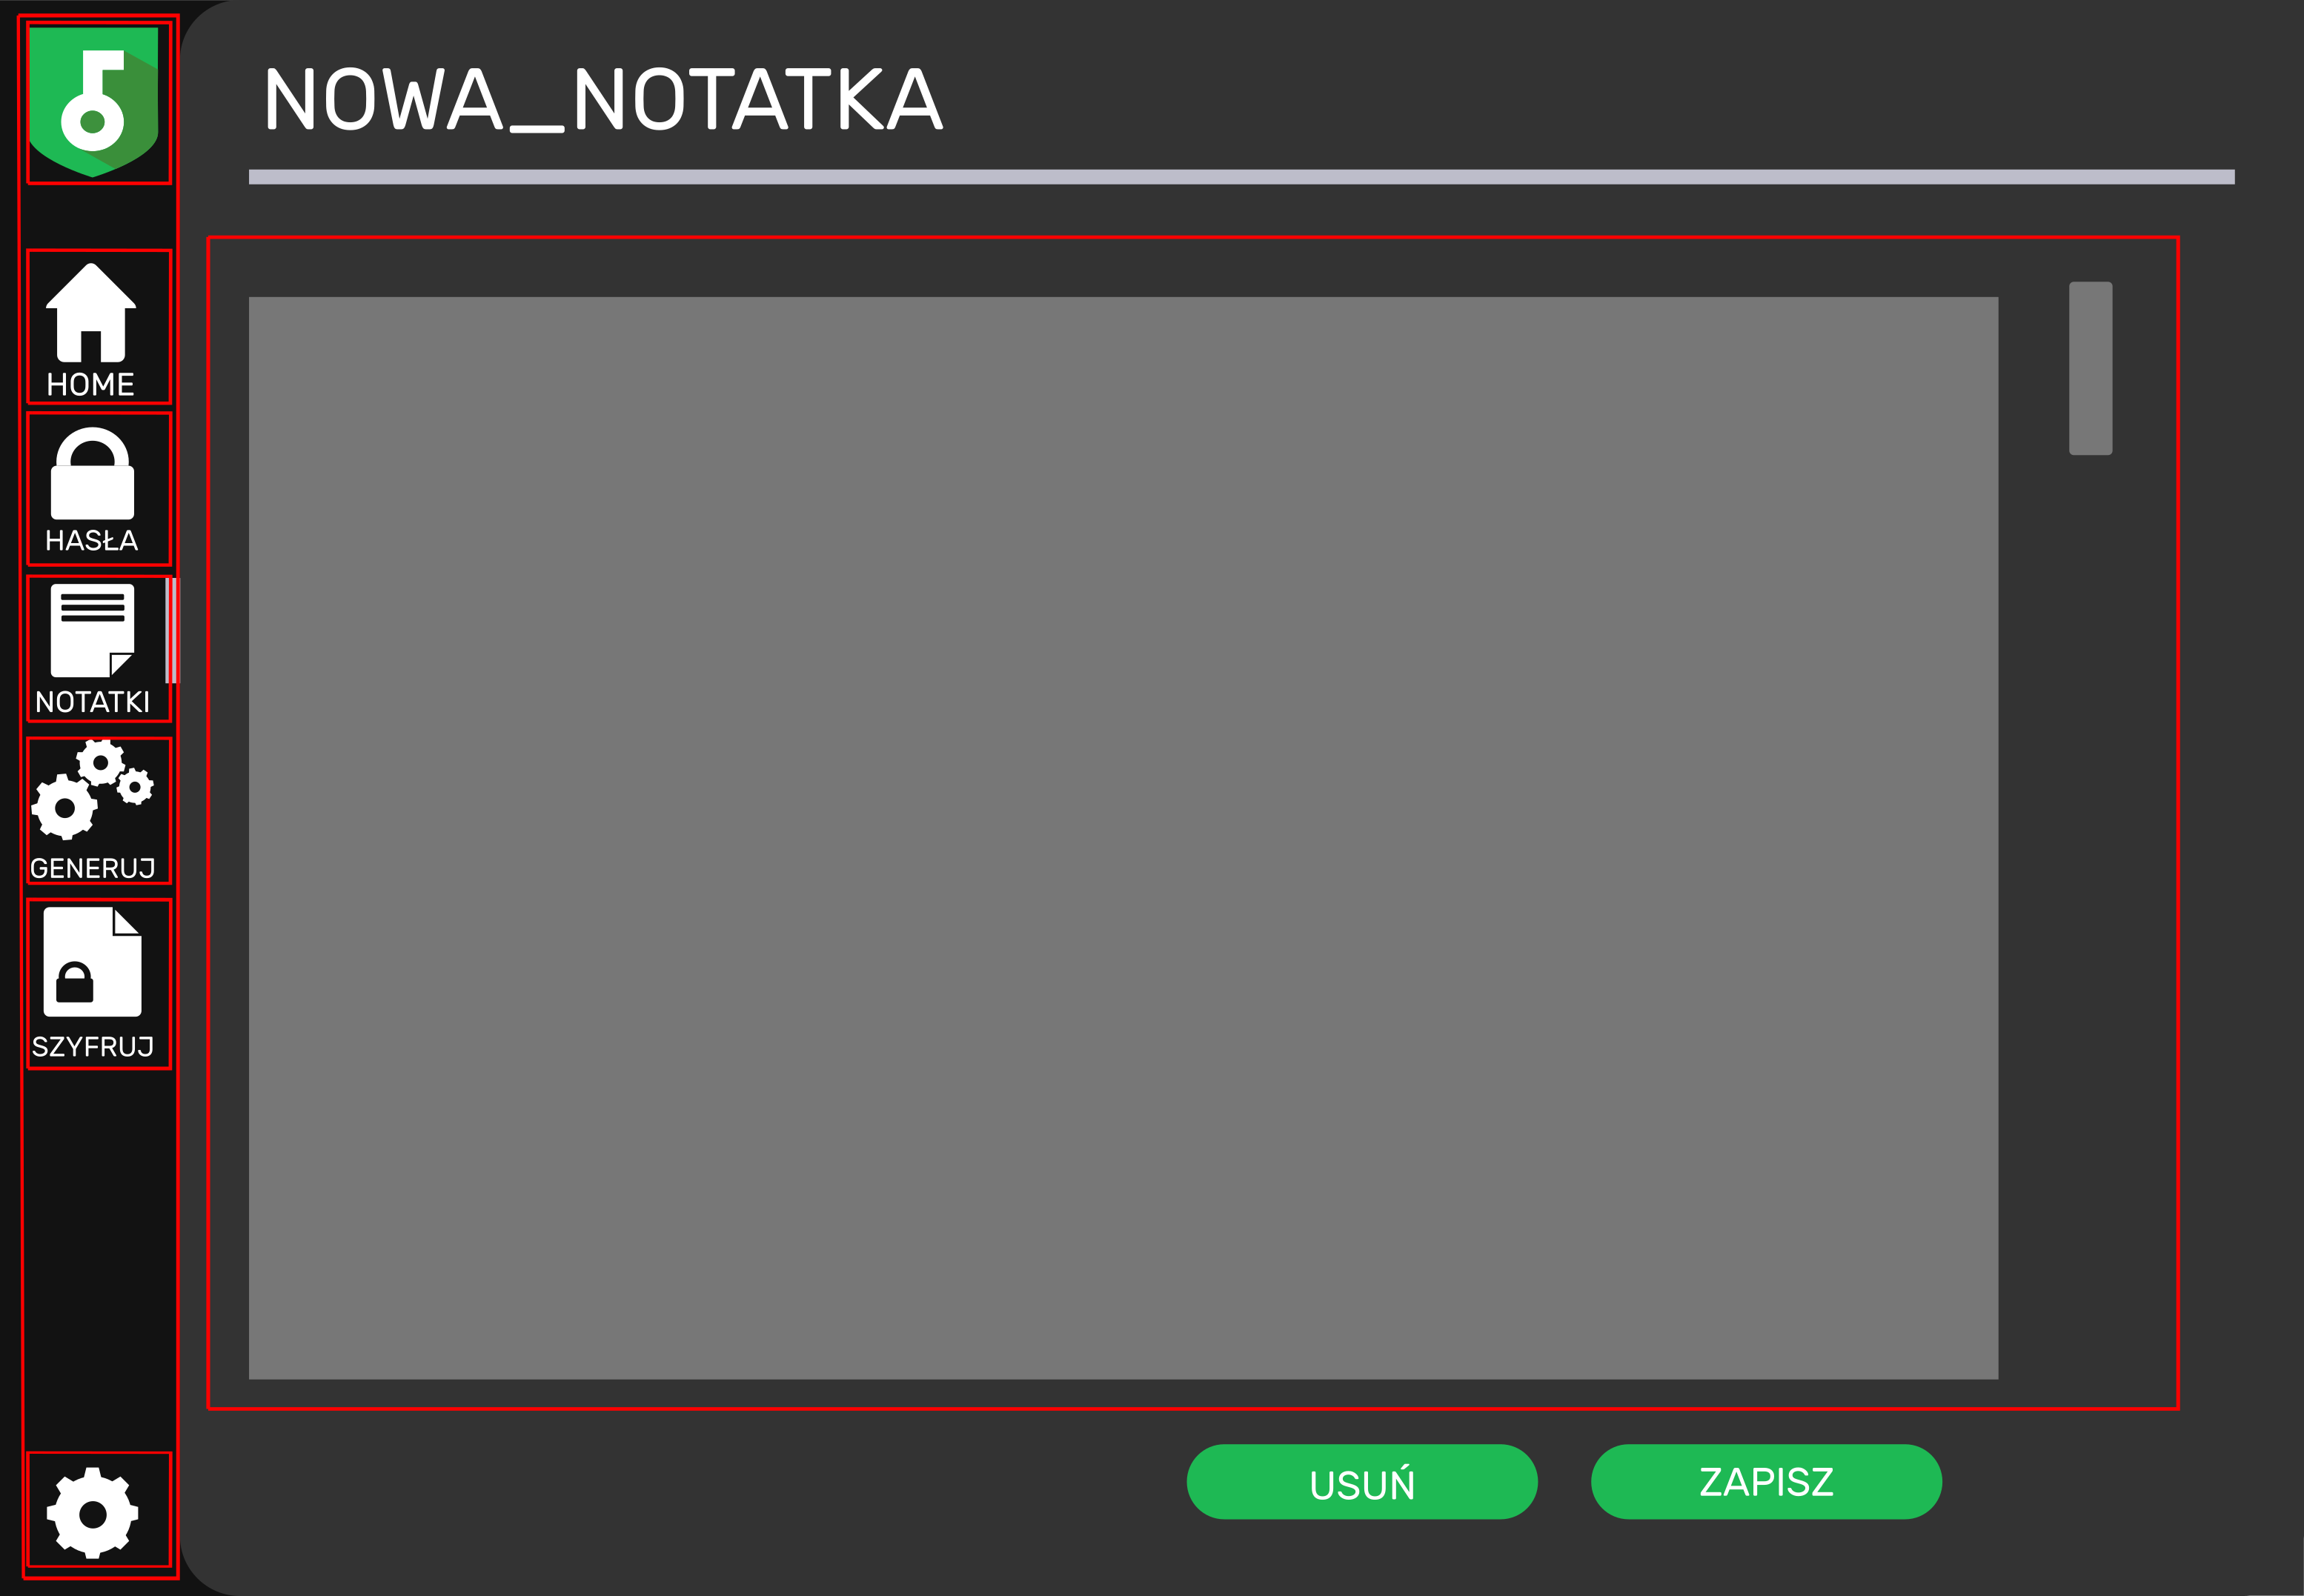
\includegraphics[width=1\textwidth]{img/ekran_nowej_not.png}
    \caption{Ekran dodawania lub edycji notatek}
    \label{fig:notatkNowe}
\end{figure}

\begin{figure}[H]
    \centering
    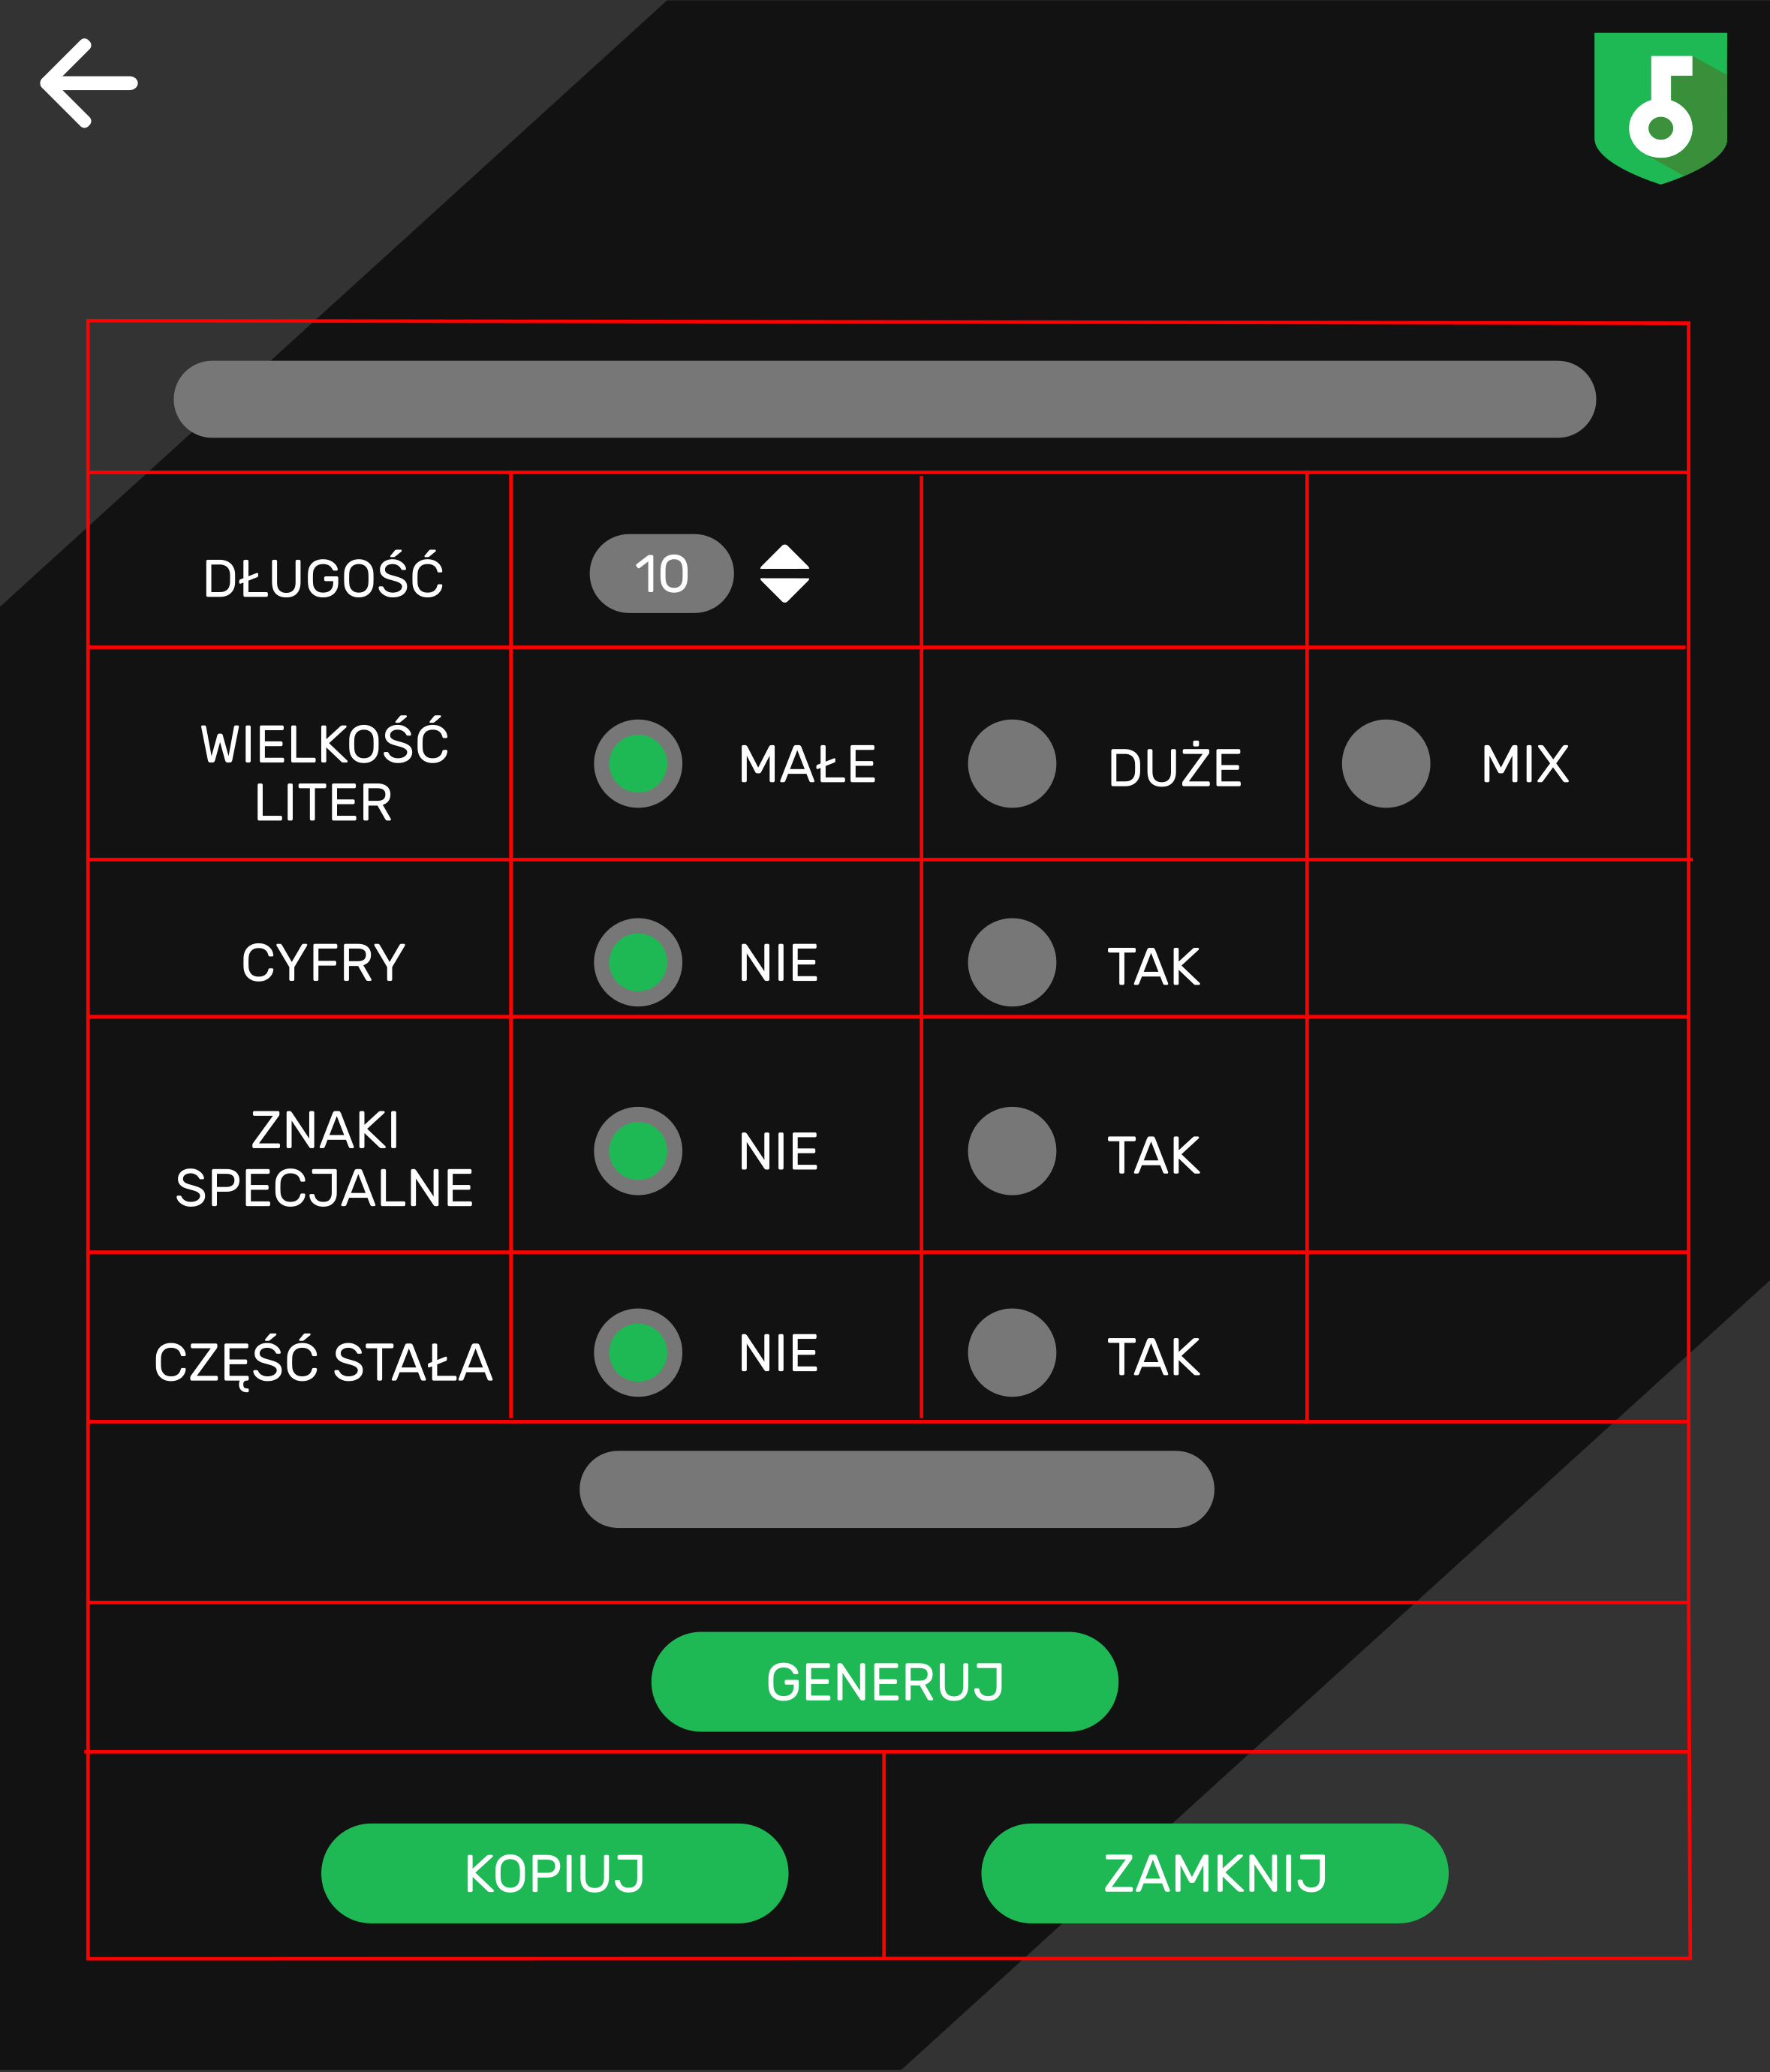
\includegraphics[width=1\textwidth]{img/ekran_generacji.png}
    \caption{Ekran szyfrowania plików podanych przez użytkownika}
    \label{fig:szyfrowanie}
\end{figure}



\section{Testowanie}
\subsection{Użyte narzędzia}
Do przetestowania kodu użyjemy narzędzi z biblioteki AssertJ. Natomiast GUI przetestujemy ręcznie podczas tworzenia aplikacji. Dodatkowo gotowy program przetestujemy sami, grając w niego oraz przekażemy go do testów znajomym.

\subsection{Konwencja}
Metody testujące przyjmą nazwy przypominające równoważniki zdań, aby w~jednoznaczny sposób przekazać informację o badaniu konkretnej funkcjonalności.

\subsection{Warunki brzegowe}
\begin{itemize}
    \item Możliwość otwarcia pliku konfiguracyjnego.
    \item Możliwość otwarcia i zapisu pliku stanu gry.
    \item Odpowiednie działanie programu w przypadku spotkania się wiązki laserowej i spadającego klocka.
    \item Odpowiednie działania programu w kontekście zliczania punktów gracza.
    \item Odpowiednie działanie programu w przypadku spotkania się statków.
\end{itemize}

\section{Diagram klas}
\begin{figure}[H]
    \centering
    \includegraphics[width=\textwidth]{img/diagram-klas.png}
    \caption{Diagram klas}
    \label{fig:diagram}
\end{figure}
\label{end}

\end{document}